% Chapter on Distributed Deep Learning.
%
% Developed for my Master Thesis at Maastricht University.
% Based on Eugenio Senes's template at the University of Torino.
%
% By Joeri Hermans (joeri@joerihermans.com)
%
% Released under an MIT license. Share, modify and enjoy, but quote the author!

\chapter{Distributed Deep Learning}
\label{chapter:distributed_deep_learning}

In this chapter, we introduce several concepts and techniques related to Distributed Deep Learning on which this works builts upon. We start in Section~\ref{sec:ddl_introduction} with a recap of all methods and techniques we have discussed in Chapter~\ref{chapter:introduction}. Afterwards, we continue with a discussion of synchronous followed by an examination of asynchronous optimization methods such as \textsc{downpour} and closely related extensions. Furthermore, we address several issues such as \emph{asynchrony induced momentum} which are related to asynchronous optimization. We also consider several approaches which provide a possible solution to these issues.

\section{Introduction}
\label{sec:ddl_introduction}

For all practical applications, Stochastic Gradient Descent (\textsc{sgd}) and derrivatives are the best tools from the numerical optimization toolbox for neural networks. However, applying \textsc{sgd} in its pure form, that is, updating the parameters after evaluating a training sample, is a computationally intensive process. An initial approach for speeding up \textsc{sgd} in terms of convergence with respect to training time was to compute the gradients of several samples, a \emph{mini-batch}, and average them. This approach has several advantages, the first being that a larger mini-batch will result in less noisy updates, as more ``evidence'' of the surrounding error space will provide a better gradient update. The second advantage being the increased computational parallelism, since all sub-gradients (gradients of the training samples in the mini-batch) are based upon the same parametrization of the model. As a result, the parallelization of the gradient computation is quite straightforward. For instance, for every training sample in a mini-batch, one could allocate a thread, a process, or even a different machine (see Figure~\ref{fig:distributed_mini_batch_parallelism}) to compute the gradients in parallel. However, a blocking mechanism is required in order to sum all gradients, average them, and finally update the parametrization of the model. This process is depicted in Figure~\ref{fig:minibatch_data_parallelism}. As discussed in Chapter~\ref{chapter:introduction}, mini-batch parallelism is an instance of \emph{synchronous data parallelism}. Although many synchronous optimization schemes share a similar structure, we discuss other instances of synchronous data parallelism in particular in Section~\ref{sec:synchronous_data_parallelism} since these optimization schemes incorperate gradients and worker parameterizations into the central variable differently compared to mini-batch parallelism.\\

Nevertheless, a significant, but albeit technical issue in synchronous optimization is when a single or multiple workers are slowed down for some reason, e.g., due to high CPU load, or bandwidth consumption, other workers will have to wait before they can continue with step $t + 1$. As a result, the allocated resources are not fully utilized. This particular issue is known in literature as the \emph{straggler} problem. However, this problem can be mitigated with by using a \emph{homogeneous} hardware configuration. For instance, when one would employ 2 different GPU's running at different clock speeds, a \emph{heteregenous} hardware configuration, then the CPU will always have to wait for a particulur GPU since it runs at a lower clock speed causing the complete training procedure to be slowed down\footnote{A chain is only as strong as its weakest link.}. Furthermore, we could argue that there is a limit to synchronous data parallelism because simply \emph{adding more workers to the problem implicitly increases the size of the mini-batch}. As a result, when applying synchronous data parallelism, one is not parallelizing gradient descent in a typical sense, but rather parallelizing the computations within a step. Of course, one could even increase the parallelism within synchronous data parallelism even further by applying model parallelism as dicussed briefly in Section~\ref{sec:intro_model_parallelism}. Nevertheless, while such an implementation is definitly possible, it might be more cost-aware from an economical perspective to just let the model train for a longer period of the compared to actually implementing the training procedure described above. Furthermore, even with if one would implement said training method, there is still a limit to the amount parallelism due to the structure of the computation graph, and communication cost between devices which have to be taken into account. This of course begs the question if it is actually possible to push the limits of asynchrony, and thereby reducing the training time even further. Or from a different perspective, is there a more trivial method besides implementing the above training procedure to reduce the training time.\\

Several approaches~\cite{dean2012large, ho2013more, cipar2013solving, recht2011hogwild, zhang2015deep, louppe2010zealous, jiang2017heterogeneity} have been suggested over the past years which accomplish exactly this. All these methods are instances of \emph{asynchronous data parallelism}, discussed in Section~\ref{sec:intro_data_parallelism}. In contrast to synchronous data parallelism, asynchronous methods can be identified by the \emph{absence} of a blocking mechanism which is present in synchronous data parallelism. Despite the fact that this method resolves the waiting time induced by stragglers, it introduces a closely related but persistent issue. More formally, the \emph{staleness} issue is due to the fact that all $n$ workers update the central variable in an asynchronous fashion. Meaning, from the moment a worker $k$ is done computing an update $\Delta\theta^k$ based upon parameterization of the central variable $\tilde{\theta}_{t}$, it will commit $\Delta\theta^k$ to the parameter server, and afterwards continue with the next mini-batch. Because of this behaviour, it is possible that a number of central variable updates $\tau$ occurred during the time worker $k$ was computing $\Delta\theta^k$. As a result, instead of obtaining $\tilde{\theta}_{t+1}$ by applying $\Delta\theta^k$, worker $k$ is actually applying $\Delta\theta^k$ to $\tilde{\theta}_{t+\tau}$. Which is not ideal, since $\Delta\theta^k$ is based on parametrization $\tilde{\theta}_t$. From~\cite{implicitmomentum} we know that increasing the number of workers actually increases the amount of staleness $\tau$ since $\mathbf{E}[\tau] = (n - 1)$ under a \emph{homogeneous} hardware configuration and a simple queuing model\footnote{With a simple queuing model we intent that updates $\Delta\theta^k$ are incorperated into the central variable in a queuing fashion.}. This result is validated empirically in one of our experiments, shown in Figure~\ref{fig:staleness_distribution}.\\

A side-effect of updating the central variable with stale updates in an asynchronous fashion, is that stale updates carry information about previous states of the central variable. Which is to be expected since worker updates are based on older parameterizations of the central variable. Using this intuition, the authors in~\cite{implicitmomentum} show formally that in a regular asynchronous \textsc{sgd} setting, like \textsc{downpour}, stale updates behave like \emph{momentum}. Furthermore, their formalization can even describe the amount of \emph{implicit momentum}, described in Equation~\ref{eq:implicit_momentum}, which is present in an asynchronous optimization procedure. Furthermore, when applying (Nesterov) momentum in a traditional optimization setting, i.e., sequential parameter updates, one needs to specify the amount of momentum. This is usually denoted by a hyperparameter $\mu$. However, we would like to note that in an asynchronous setting, the hyperparameter $\mu_s$ from Equation~\ref{eq:implicit_momentum}, is not explicitly defined in the optimizer, but arises from the number of asynchronous workers. As a result, Equation~\ref{eq:implicit_momentum} is merely descriptive.

\begin{equation}
  \label{eq:implicit_momentum}
  \mu_s = \Bigg(1 - \frac{1}{n}\Bigg)
\end{equation}

In a previous paragraph we said that there is a limit to mini-batch parallelism, since adding more workers to the problem implicitly increases the size of a mini-batch. However, we observe in Figure~\ref{fig:staleness_distribution} in accordance with~\cite{implicitmomentum}, that there might be a limit to asynchronous optimization as well. However, the authors in~\cite{implicitmomentum} assume that gradients coming from the workers are not adaptive\footnote{Meaning, they are not modified with respect to some (hyper)parameter.}, as can be detucted from their proof. The question begs, can we push asynchronous optimization even further? We answer this question in Chapter~\ref{chapter:accumulated_gradient_normalization}, and Chapter~\ref{chapter:asynchronous_distributed_adaptive_gradients}, by introducing new techniques using a better, and more intuitive understanding of parameter staleness.

\begin{figure}
  \centering
  \begin{subfigure}{.45\textwidth}
    \centering
    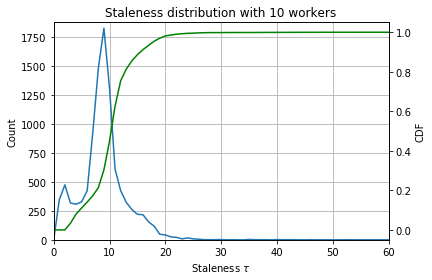
\includegraphics[width=\linewidth]{resources/images/staleness_10}
    \caption{$n = 10$}
    \label{fig:staleness_distribution_10}
  \end{subfigure}
  \begin{subfigure}{.45\textwidth}
     \centering
     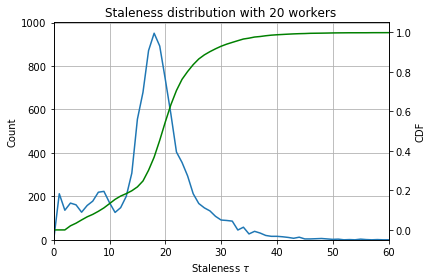
\includegraphics[width=\linewidth]{resources/images/staleness_20}
     \caption{$n = 20$}
    \label{fig:staleness_distribution_20}
  \end{subfigure}
  \begin{subfigure}{.45\textwidth}
     \centering
     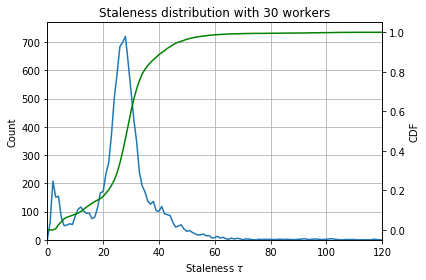
\includegraphics[width=\linewidth]{resources/images/staleness_30}
     \caption{$n = 30$}
     \label{fig:staleness_distribution_30}
  \end{subfigure}
  \begin{subfigure}{.45\textwidth}
     \centering
     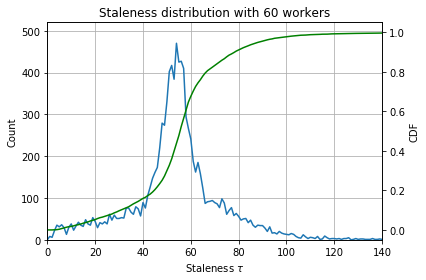
\includegraphics[width=\linewidth]{resources/images/staleness_60}
     \caption{$n = 60$}
     \label{fig:staleness_distribution_60}
  \end{subfigure}
  \caption{These figures show the staleness distribution during a training procedure using a differing number of parallel workers. For every central variable update, we record the staleness $\tau$, and increment the number of occurences of this particular staleness by 1. Thus effectievely building a histogram showing the staleness distribution during the training. With this, we experimentally validate the observations of~\cite{implicitmomentum} that $\mathbf{E}[\tau] = (n - 1)$. Furthermore, the claim that staleness is geometrically distributed during training also holds (right half of the distribution).}
  \label{fig:staleness_distribution}
\end{figure}

\section{Synchronous Data Parallelism}
\label{sec:synchronous_data_parallelism}

\subsection{Model Averaging}
\label{sec:model_averaging}

As the name suggests, model averaging optimizes the central variable by simply averaging the parametrizations of the workers after $\lambda$ (which could be the amount of data in a single epoch) steps until all data has been consumed. As mentioned before, hyperparameter $\lambda$ denotes the number of \emph{local} steps that have to be performed before the results are communicated with the parameter server. The optimization procedure in the worker and parameter server are quite straightforward, and are described in Equation~\ref{eq:model_averaging_worker_update} and Equation~\ref{eq:model_averaging_ps_update} respectively. However, Equation~\ref{eq:model_averaging_worker_update} has the disadvantage that a lot of communication with the parameter server has to be performed, since after every \emph{local} worker update all parameters have to be shipped to the parameter server to apply Equation~\ref{eq:model_averaging_ps_update}. Furthermore, this approach has several other issues that will be discussed later. But for now we can resolve this issue by delaying a commit to the parameter server by doing several \emph{local} ($\lambda$) updates before sending $\theta^k_t$ to the parameter server, this is shown in Algorithm~\ref{algo:model_averaging_worker}.

\begin{equation}
  \label{eq:model_averaging_worker_update}
  \theta^k_{t+1} = \theta^k_t - \eta_t \odot \nabla_\theta \mathcal{L}(\theta^k_t;\textbf{x}^k_t;\textbf{y}^k_t)
\end{equation}

\begin{equation}
  \label{eq:model_averaging_ps_update}
  \tilde{\theta}_{t+1} = \frac{1}{n}\sum^n_{i=1} \theta^i_t
\end{equation}

Contrary to other synchronous methods, model averaging does not reduce the training time in general. In fact, it requires more resources to achieve the same results since the central variable is set to be the average of all workers. This is shown in Figure~\ref{fig:model_averaging_slow} (a) since all workers follow the same first-order path, synchronize, and average the parameters after $\lambda$ steps to start again from the averaged parameterization, which is in this case the central variable. However, what happens if we initialize the parameterizations of the workers randomly? At first, all workers will do some work locally, but after $\lambda$ steps, the parametrizations of the workers are averaged. As a result, all workers share the same parameterization in the next step, which brings us again to our initial scenario as shown in Figure~\ref{fig:model_averaging_slow} (b). Furthermore, when applying random initialization, we could say a ``warmup'' period is required since all workers need to converge a particular solution before convergence can take place. This intuition is strenghtened in Figure~\ref{fig:model_averaging_intuition}.

\begin{figure}[H]
  \centering
  \begin{subfigure}{.49\textwidth}
    \centering
    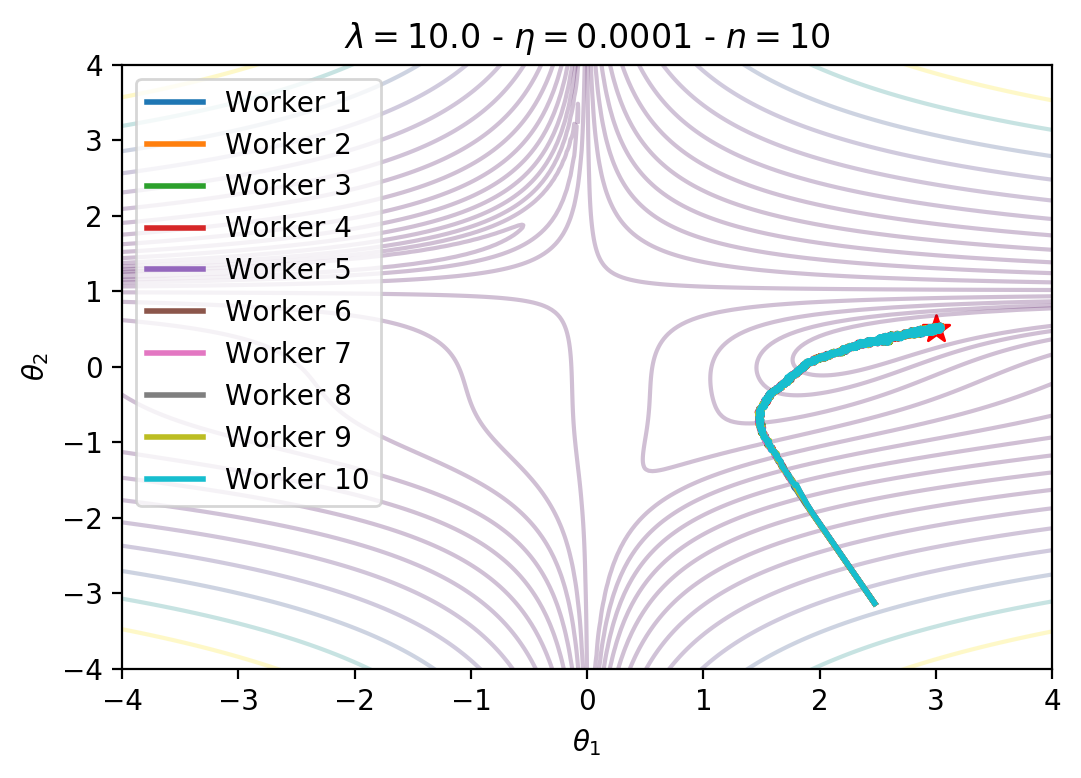
\includegraphics[width=\linewidth]{resources/images/model_averaging_identical_starting_point}
    \caption{Identical initialization}
  \end{subfigure}
  \begin{subfigure}{.49\textwidth}
    \centering
    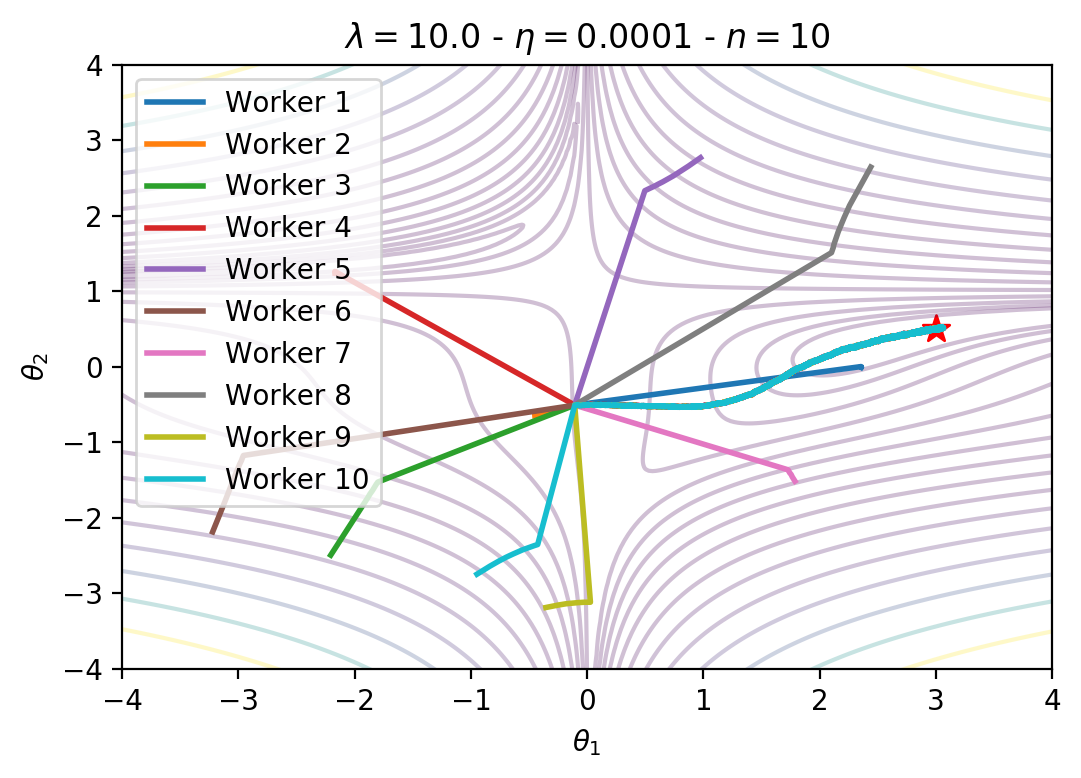
\includegraphics[width=\linewidth]{resources/images/model_averaging_cf_10}
    \caption{Random initialization}
  \end{subfigure}
  \caption{In this Figure we show the difference between identical initialization (a), and random initialization (b). In essence, both methods require roughly the same amount of time as a sequential optimization algorithm, i.e., not distributed, while using more resources. However, the difference here is that using random initialization requires a ``warmup'' period (a single parameter server update), before the actual optimization process can start. In order to simulate the stochastic noise of mini-batch gradient descent, we added a noise term to our gradient computations which was sampled from $X \sim \mathcal{N}(\mu = 0,\,\sigma^{2} = 10.0)$ to ensure that some deviation from the central variable was possible.}
  \label{fig:model_averaging_slow}
\end{figure}

\newpage

\begin{algorithm}[H]
  \caption{Describes the worker procedure with local worker exploration. The worker will be identified with a certain index $k$ and will be initialized by assigning the central variable ($\tilde{\theta}_t$) to the worker, or the worker variable can be randomized at the start of the optimization procedure. Furthermore, we introduce a hyperparameter $\lambda$, which is the number of local updates that have to be performed in order the worker parameterization $\theta^k_t$ is communicated with the parameter server.}
  \label{algo:model_averaging_worker}
  \begin{algorithmic}[1]
    \Procedure{ModelAveragingWorker}{$k$}
    \State $\theta^k_0 \gets \Call{Pull()}{}$ or $\Call{Random()}{}$ \Comment{Worker variable $\theta^k_0$ can be randomized.}
    \State $t \gets 0$
    \While{$\textbf{not}$ converged}
    \State $i \gets 0$
    \For{$i < \lambda$}
    \State $\textbf{x},~\textbf{y} \gets \Call{FetchNextMiniBatch()}{}$
    \State $\theta^k_{t + 1} \gets \theta^k_t - \eta_t \odot \nabla_\theta \mathcal{L}(\theta^k_t;\textbf{x};\textbf{y})$ \Comment{Optimization step, could be \cite{kingma2014adam}, or other optimizer.}
    \State $i \gets i + 1$
    \State $t \gets t + 1$
    \EndFor
    \State $\Call{Commit}{\theta^k_t}$
    \State $\Call{WaitForOtherWorkers()}{}$
    \State $\theta^k_t \gets \Call{Pull()}{}$
    \EndWhile
    \EndProcedure
  \end{algorithmic}
\end{algorithm}

\vspace*{1cm}

\begin{figure}[H]
  \centering
  %% 1
  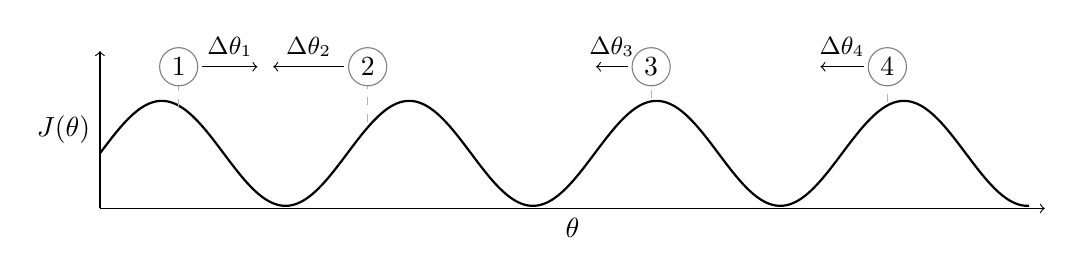
\begin{tikzpicture}
    % Draw the axis of the plots.
    \draw[->] (0,0) -- (12,0) node[midway, below] {$\theta$};
    \draw[->] (0,0) -- (0, 2) node[midway, left] {$J(\theta)$};
    % Draw the hypothesis space, which is sin(x) / 2 + 0.55
    \draw[samples=400,domain=0:11.8,smooth,variable=\x,black,thick]  plot ({\x},{sin(deg(\x * 2)) / 1.5 + 0.7});
    % Draw the instances, and their gradient arrows.
    \draw (1,1.8) node[circle,inner sep=2pt,draw=black!50] {1};
    \draw[dashed, draw=black!30] (1,1.28) -- (1,1.55);
    \draw[->] (1.3,1.8) -- (2,1.8) node[midway, above] {\small $\Delta\theta_1$};

    \draw (3.4,1.8) node[circle,inner sep=2pt,draw=black!50] {2};
    \draw[dashed, draw=black!30] (3.4,1.1) -- (3.4,1.55);
    \draw[->] (3.1,1.8) -- (2.2,1.8) node[midway, above] {\small $\Delta\theta_2$};

    \draw (7,1.8) node[circle,inner sep=2pt,draw=black!50] {3};
    \draw[dashed, draw=black!30] (7,1.4) -- (7,1.55);
    \draw[->] (6.7,1.8) -- (6.3,1.8) node[midway, above] {\small $\Delta\theta_3$};

    \draw (10,1.8) node[circle,inner sep=2pt,draw=black!50] {4};
    \draw[dashed, draw=black!30] (10,1.35) -- (10,1.55);
    \draw[->] (9.7,1.8) -- (9.15,1.8) node[midway, above] {\small $\Delta\theta_4$};
  \end{tikzpicture}
  %% 2
  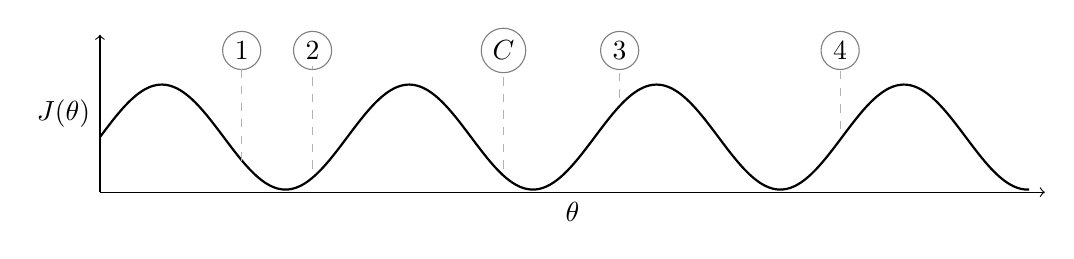
\begin{tikzpicture}
    % Draw the axis of the plots.
    \draw[->] (0,0) -- (12,0) node[midway, below] {$\theta$};
    \draw[->] (0,0) -- (0, 2) node[midway, left] {$J(\theta)$};
    % Draw the hypothesis space, which is sin(x) / 2 + 0.55
    \draw[samples=400,domain=0:11.8,smooth,variable=\x,black,thick]  plot ({\x},{sin(deg(\x * 2)) / 1.5 + 0.7});
    % Draw the instances, and their gradient arrows.
    \draw (1.8,1.8) node[circle,inner sep=2pt,draw=black!50] {1};
    \draw[dashed, draw=black!30] (1.8,0.4) -- (1.8,1.6);

    \draw (2.7,1.8) node[circle,inner sep=2pt,draw=black!50] {2};
    \draw[dashed, draw=black!30] (2.7,0.3) -- (2.7,1.6);

    \draw (6.6,1.8) node[circle,inner sep=2pt,draw=black!50] {3};
    \draw[dashed, draw=black!30] (6.6,1.2) -- (6.6,1.6);

    \draw (9.4,1.8) node[circle,inner sep=2pt,draw=black!50] {4};
    \draw[dashed, draw=black!30] (9.4,0.8) -- (9.4,1.6);
    % Draw the center variable.
    \draw (5.125,1.8) node[circle,inner sep=2pt, draw=black!50] {$C$};
    \draw[dashed, draw=black!30] (5.125,0.3) -- (5.125,1.5);
  \end{tikzpicture}
  %% 3
  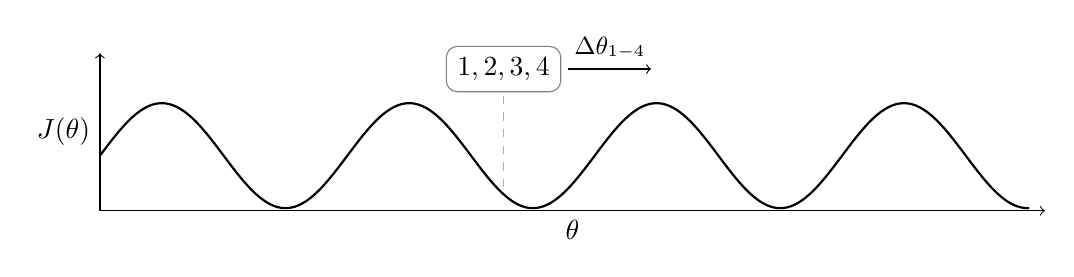
\begin{tikzpicture}
    % Draw the axis of the plots.
    \draw[->] (0,0) -- (12,0) node[midway, below] {$\theta$};
    \draw[->] (0,0) -- (0, 2) node[midway, left] {$J(\theta)$};
    % Draw the hypothesis space, which is sin(x) / 2 + 0.55
    \draw[samples=400,domain=0:11.8,smooth,variable=\x,black,thick]  plot ({\x},{sin(deg(\x * 2)) / 1.5 + 0.7});
    % Draw the instances, and their gradient arrows.
    \draw (5.125,1.8) node[rectangle,rounded corners,inner sep=4pt, draw=black!50] {$1,2,3,4$};
    \draw[dashed, draw=black!30] (5.125,0.3) -- (5.125,1.5);
    \draw[->] (5.95,1.8) -- (7,1.8) node[midway, above] {\small $\Delta\theta_{1-4}$};
  \end{tikzpicture}
  \caption{This figure explains the intuition behind model averaging. In the first state, all workers, $w_1$, $w_2$, $w_3$, and $w_4$, are uniformly initialized over the hypothesis space. Using the local parametrizations, every worker obtains an update $\Delta w_i$, and applies it locally. Afterwards, all workers send their parametrizations to the parameter server which will average them to obtain a central variable, which is depicted by $C$ in this particular figure. Finally, all workers fetch the most recent central variable, and start computing new gradients based for the following iteration.  Furthermore, what can be observed directly from this figure, is that when the workers do not agree on a \emph{local neighborhood}, the central variable will not be able to converge. This is additional support for Hypothesis~\ref{hyp:local_optimization}.}
  \label{fig:model_averaging_intuition}
\end{figure}

Nevertheless, what is interesting about the random initialization of workers, is that when we increase the number of workers, the probability that we will find a better solution (minima) compared to a sequential optimization process increases. However, this also depends on the curvature of the error space. For example, in Figure~\ref{fig:model_averaging_prob} we use Beale's function to obtain our statistic. However, from the plots we can deduce that the curvature of the error space is slightly biased towards the global minimum if first-order gradients are used. If the error space was not biased towards a specific minima, the statistic for a single worker under different hyperparameterizations should be 50\%.\\

Furthermore, what is the role of the exploration parameter $\lambda$? Does it contribute to to the optimization process besides reducing the amount of communication with the parameter server by increasing the amount of local work? In principle this would help to optimization process since more exploration of the parameter space occurs, and as a result, better updates are applied. Furthermore, remember what we said in Section~\ref{sec:ddl_introduction} on synchronous data parallelism, that effectivly increasing the number of workers implicitly increases the size of the mini-batch. Yet, in this particular case there is a subtle difference, i.e., local exploration of the parameter space. As a result, it is not implicitly increasing the size of the mini-batch since some form of local exploration occurs. As a result, \emph{the averaged central variable will produce a less-noisy consensus based on the (local) exploration of the error space}.  However, the problem lies in the fact when different sets of workers enter different minima, possibly because of \emph{too much exploration of the error space}, as depicted in Figure~\ref{fig:model_averaging_intuition}. Because if this happens, then the averaging step could potentially reset the situation instead of continuing exploring a single minima.

\begin{figure}
  \centering
  \begin{subfigure}{.35\textwidth}
    \centering
    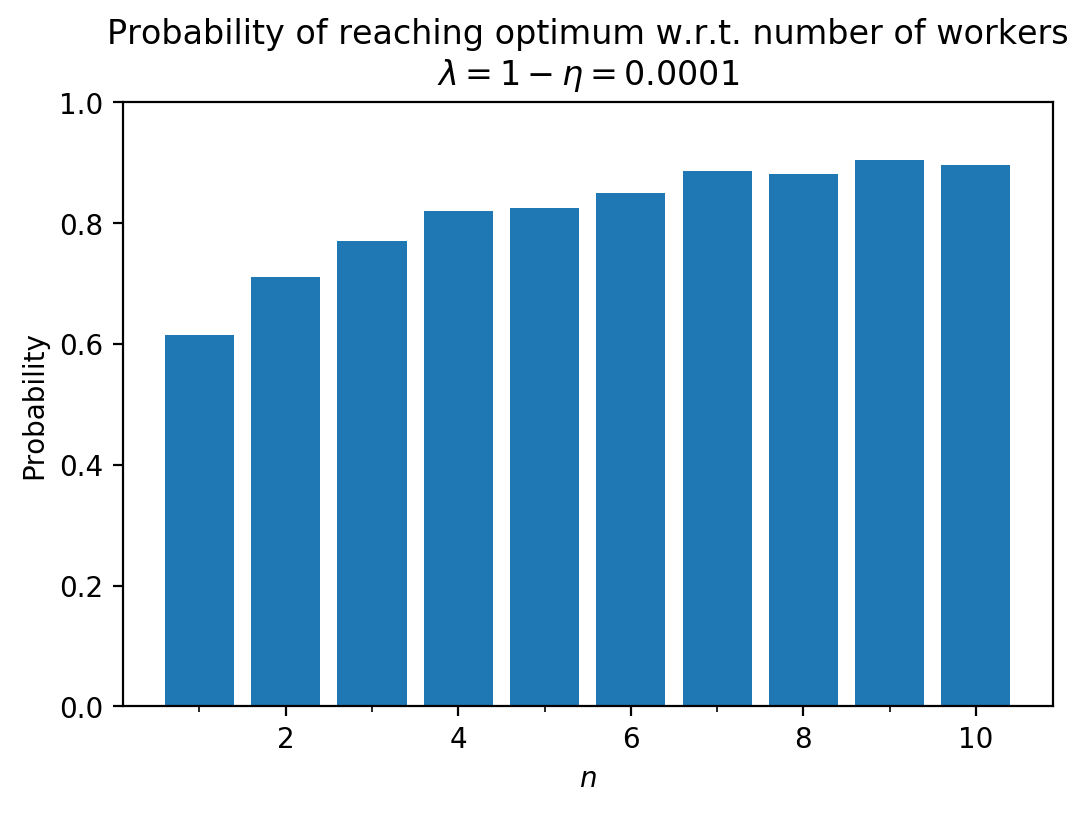
\includegraphics[width=\linewidth]{resources/images/model_averaging_prob_1}
    \caption{$\lambda = 1$}
  \end{subfigure}
  \begin{subfigure}{.35\textwidth}
    \centering
    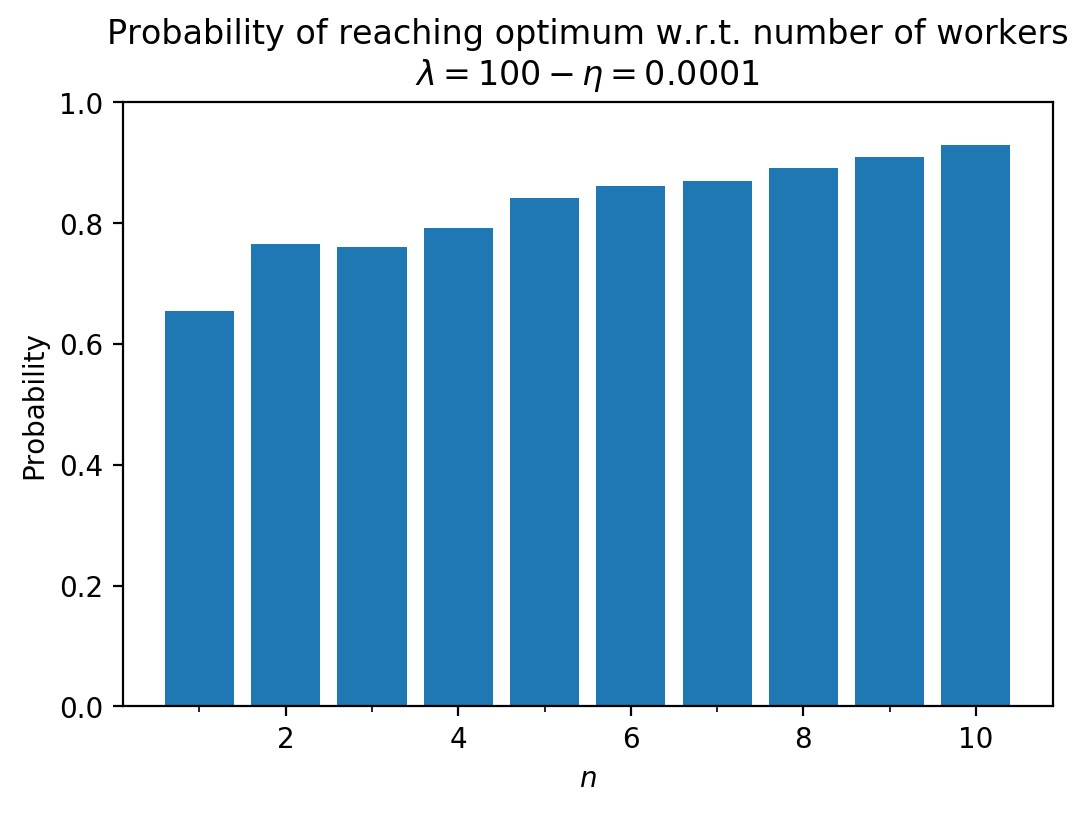
\includegraphics[width=\linewidth]{resources/images/model_averaging_cf_100_prob}
    \caption{$\lambda = 100$}
  \end{subfigure}
  \caption{Probability distribution extracted from several Monte-Carlo simulations under different conditions. We find that the probability of reaching the optimum (Beale's function) increases when the number of random initialized workers increases. Despite the fact that we observe that more exploration ($\lambda$) yiels a better statistic, we believe that this result is not significant due to the relatively low number of simulations (1000 per worker per hyperparameter).}
  \label{fig:model_averaging_prob}
\end{figure}

\begin{figure}[H]
  \centering
  \begin{subfigure}{.24\textwidth}
    \centering
    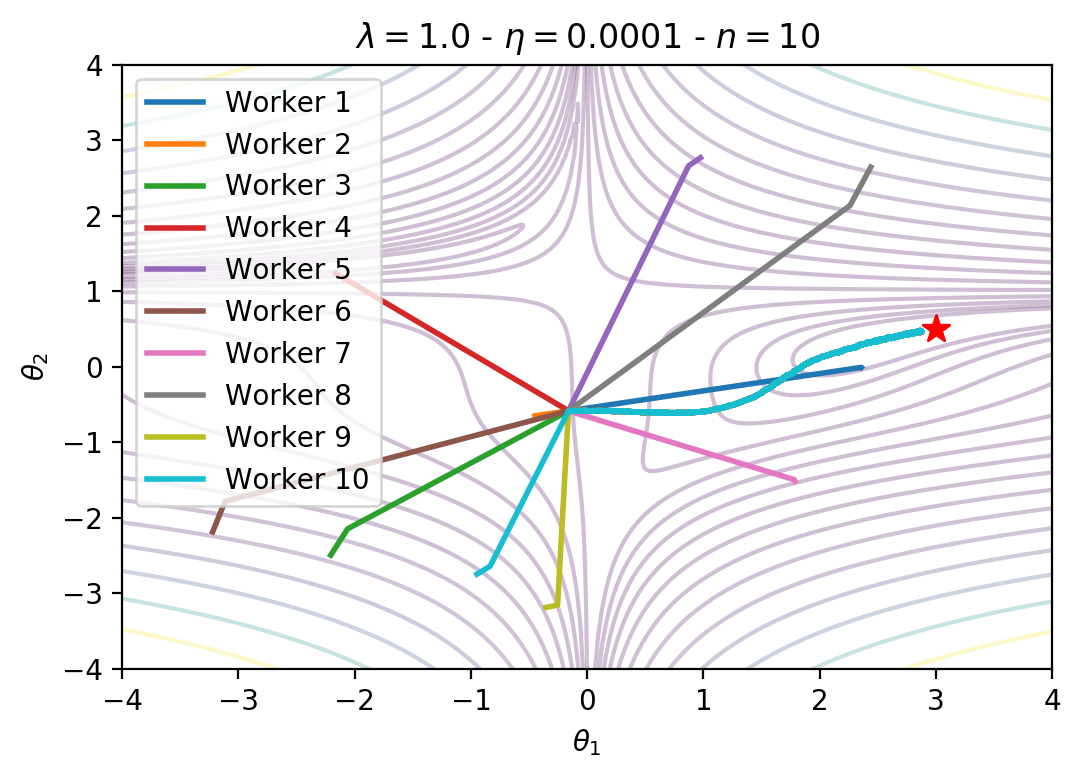
\includegraphics[width=\linewidth]{resources/images/model_averaging_cf_1}
    \caption{$\lambda = 1$}
  \end{subfigure}
  \begin{subfigure}{.24\textwidth}
    \centering
    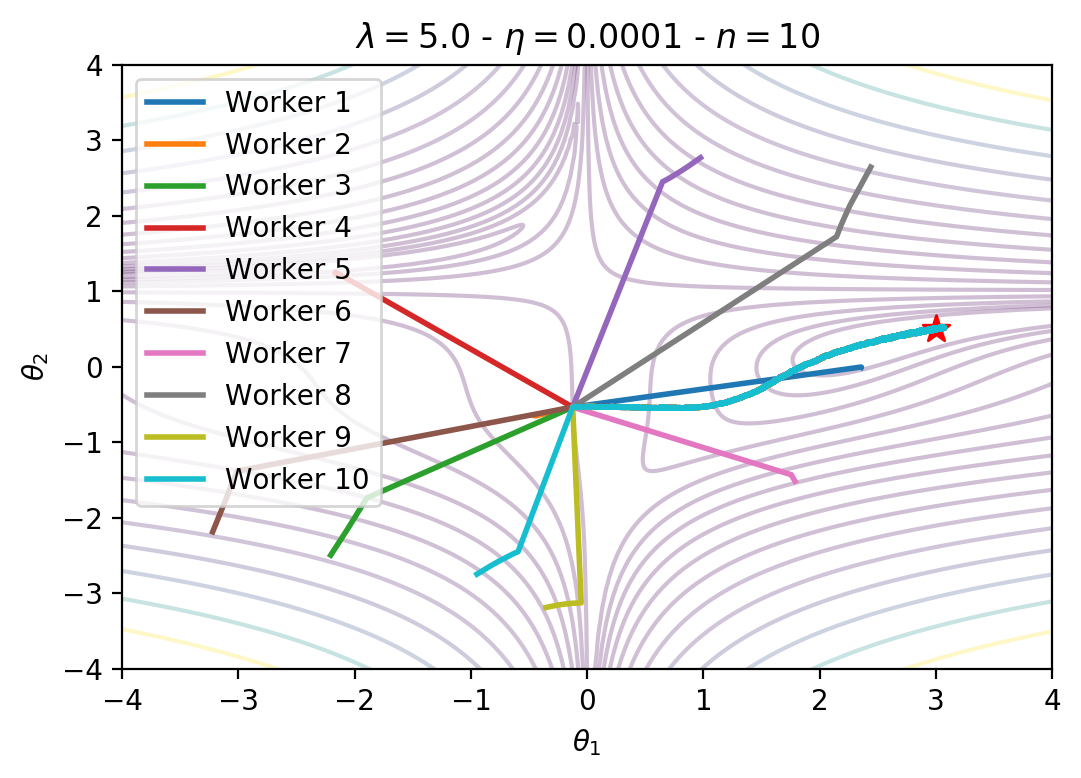
\includegraphics[width=\linewidth]{resources/images/model_averaging_cf_5}
    \caption{$\lambda = 5$}
  \end{subfigure}
  \begin{subfigure}{.24\textwidth}
    \centering
    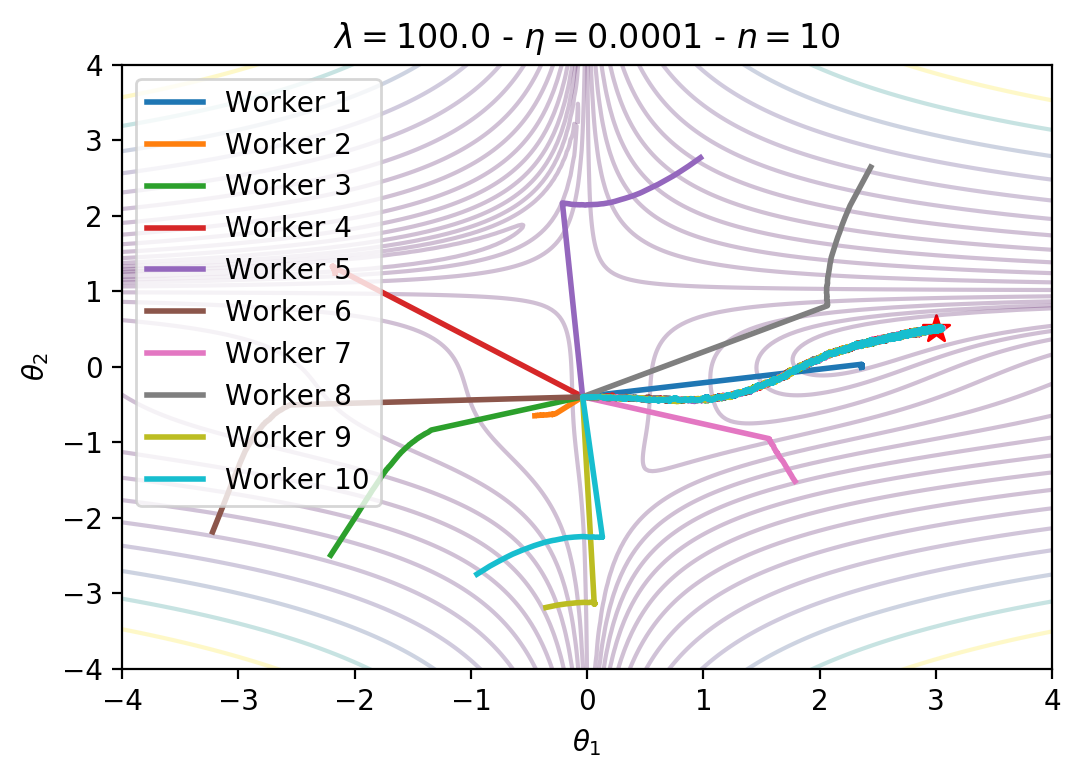
\includegraphics[width=\linewidth]{resources/images/model_averaging_cf_100}
    \caption{$\lambda = 100$}
  \end{subfigure}
  \begin{subfigure}{.24\textwidth}
    \centering
    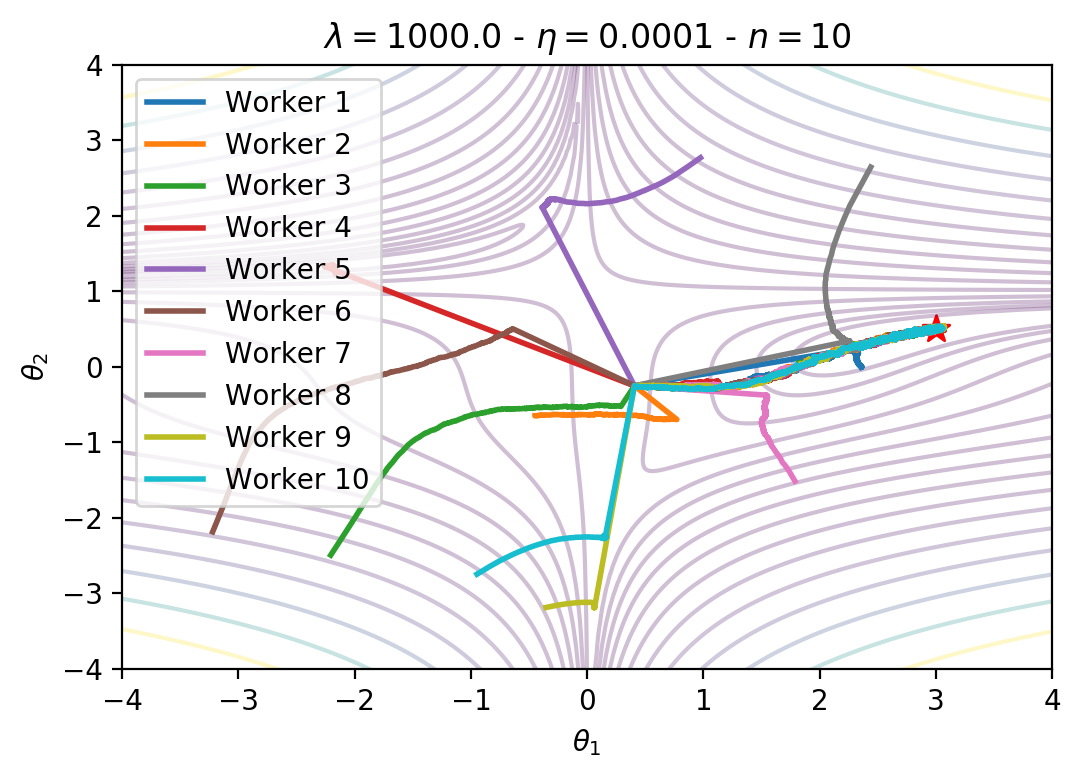
\includegraphics[width=\linewidth]{resources/images/model_averaging_cf_1000}
    \caption{$\lambda = 1000$}
  \end{subfigure}
  \label{fig:model_averaging_cf}
  \caption{Workers which have been randomly initialized (experiments use same initialization) with different values for $\lambda$ (communication frequency, or number of local worker iterations). Since the workers are initially randomized of the hypothesis space, the central variable in the first averaging step will be shifted towards the global minima because of the amount of local exploration, and due to the bias of the error space as shown in Figure~\ref{fig:model_averaging_prob}.}
\end{figure}

\subsection{Elastic Averaging SGD}
\label{sec:easgd}

Elastic Averaging SGD, or \textsc{easgd}~\cite{zhang2015deep}, is a distributed optimization algorithm designed with communication constraints in mind. In essence, \textsc{easgd} could be viewed as an extension of model averaging described in Section~\ref{sec:model_averaging} with the difference that the workers, and the central variable are coordinated using an \emph{elastic force}~\cite{zhang2015deep} instead of averaging the workers after a fixed amount of steps. This means that instead of simply transmitting the parametrization or a gradient to the parameter server, the workers commit an \emph{elastic difference} which is defined as $\eta_t \rho (\theta^k_t - \tilde{\theta}_t)$ where $\rho$ is the \emph{elasticity} hyperparameter. Intuitively, $\rho$ describes the amount of exploration that can be performed by the workers with respect to the central variable $\tilde{\theta}_t$.\\

Assuming $\lambda = 1$, the worker update and central variable update are described in Equation~\ref{eq:easgd_sync_worker}, and Equation~\ref{eq:easgd_sync_ps} respectively. What is different compared to most other optimization schemes, is that the worker update described in Equation~\ref{eq:easgd_sync_worker} has a second component, i.e., the \emph{elastic difference}. Furthermore, note that compared to other distributed optimization schemes, the workers in \textsc{easgd} do not synchronize their parameterization with the central variable as shown in Algorithm~\ref{algo:easgd_worker}, but rather update the central variable using the elastic difference, and than use the new central variable as a new reference point to compute the following elastic differences.

\begin{equation}
  \label{eq:easgd_sync_worker}
  \theta^k_{t + 1} = \theta^k_t - \eta_t \odot \nabla_\theta \mathcal{L}(\theta^k_t;\mathbf{x}^k_t;\mathbf{y}^k_t) - \eta_t\rho(\theta^k_t - \tilde{\theta}_t)
\end{equation}

\begin{equation}
  \label{eq:easgd_sync_ps}
  \tilde{\theta}_{t+1} = \tilde{\theta}_t + \eta_t \sum_{i=0}^n \rho(\theta^i_t - \tilde{\theta}_t)
\end{equation}

\begin{figure}[H]
  \centering
  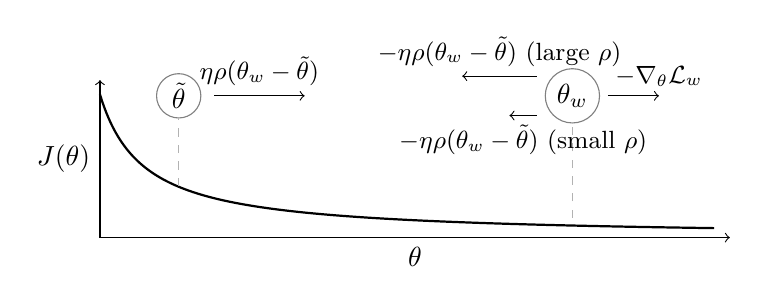
\begin{tikzpicture}
    % Draw the axis of the plots.
    \draw[->] (1,0) -- (9,0) node[midway, below] {$\theta$};
    \draw[->] (1,0) -- (1,2) node[midway, left] {$J(\theta)$};
    % Draw the function.
    \draw[samples=400,domain=1:8.8,smooth,variable=\x,black,thick]  plot ({\x},{(1 / (\x - 0.45))});
    % Draw the instances (including the center variable) with the gradient arrows and the elastic difference.
    \draw (2, 1.8) node[circle, inner sep=2pt, draw=black!50] {$\tilde{\theta}$};
    \draw[dashed, draw=black!30] (2,0.65) -- (2,1.5);
    \draw (7, 1.8) node[circle, inner sep=2pt, draw=black!50] {$\theta_w$};
    \draw[dashed, draw=black!30] (7,0.25) -- (7,1.45);
    % Draw the gradients and the elastic force.
    \draw[->] (7.45,1.8) -- (8.1,1.8) node[right, above] {\small $-\nabla_\theta \mathcal{L}_w$};
    \draw[->] (6.55,1.55) -- (6.2,1.55) node[midway, below] {\small $-\eta\rho(\theta_w - \tilde{\theta})$ (small $\rho$)};
    \draw[->] (6.55,2.05) -- (5.6,2.05) node[midway, above] {\small $-\eta\rho(\theta_w - \tilde{\theta})$ (large $\rho$)};
    % Draw elastic force applied to the central variable.
    \draw[->] (2.45, 1.8) -- (3.6, 1.8) node[midway, above] {\small $\eta\rho(\theta_w - \tilde{\theta})$};
  \end{tikzpicture}
  \caption{In this example we would like to make the intuition behind Elastic Averaging SGD clear by describing it as a classical physics problem. In this particular figure we have 1 worker, $\theta_w$ ($n = 1$, $\lambda = 1$), and a central variable $\tilde{\theta}$. The $y$-axis represents the error with respect to a certain parameterization $\theta$. Using Algorithm~\ref{algo:easgd_worker}, the worker performs $\lambda$ steps to compute the next value of $\theta_w$ using Equation~\ref{eq:easgd_sync_worker}. As stated before in Section~\ref{sec:easgd}, Equation~\ref{eq:easgd_sync_worker} holds 2 components, i.e., the regular negated first-order gradient ($-\eta_t \nabla_\theta \mathcal{L}_w$), and the \emph{negated} elastic difference ($-\eta_t\rho(\theta_w - \tilde{\theta})$). As always, the negated first-order gradient represents the steepest slope with respect to the current error (loss), and parameterization. However, the \emph{negated} elastic difference actually points towards the central variable. The magnitude of the elastic difference is controlled by hyperparameter $\rho$. This implies that a large value of $\rho$ \emph{strongly} limits the amount of exploration a worker can perform with respect to the central variable since the magnitude of the elastic difference vector will be proportionally larger compared to a small $\rho$. Finally, the central variable is updated using Equation~\ref{eq:easgd_sync_ps} and the elastic difference coming from all workers. Furthermore, we would like to note that the elastic difference during the central variable update is \emph{not} negated. Meaning that the central variable is optimized with respect to the ``pull'' of all workers, with the effect that workers whichare ahead in the optimization process, will have a larger elastic force, causing the central variable to be influenced more strongly by distant workers. Nevertheless, at the same time, distant workers are pulled towards the central variable using an equal but opposite force \emph{and} the negated gradient, i.e., the net force of the elastic difference and the negated gradient combined results either in a step towards a minimum, a null-operation, or a step in the direction of the central variable.}
  \label{fig:easgd_sync}
\end{figure}

\begin{algorithm}[H]
  \caption{Worker procedure of synchronous \textsc{easgd}. This algorithms accepts several hyperparameters, the first being the number of local computations $\lambda$, the exploration hyperparameter $\rho$, and the dynamic learning rate $\eta_t$.}
  \label{algo:easgd_worker}
  \begin{algorithmic}[1]
    \Procedure{EASGDWorker}{$k$}
    \State $\theta^k_0 \gets \tilde{\theta} \gets \Call{Pull}$
    \State $t \gets 0$
    \While{$\textbf{not}$ converged}
    \State $i \gets 0$
    \For{$i < \lambda$}
    \State $\textbf{x},~\textbf{y} \gets \Call{FetchNextMiniBatch()}{}$
    \State $\theta^k_{t + 1} \gets \theta^k_t - \eta_t \odot \nabla_\theta \mathcal{L}(\theta^k_t;\textbf{x};\textbf{y})$
    \State $i \gets i + 1$
    \State $t \gets t + 1$
    \EndFor
    \State $\mathcal{E} = \eta_t\rho(\theta^k_t - \tilde{\theta})$
    \State $\theta^k_{t+1} = \theta^k_t - \mathcal{E}$
    \State $\Call{Commit}{\mathcal{E}}$
    \State $\Call{WaitForOtherWorkers()}{}$
    \State $\tilde{\theta} \gets \Call{Pull}$
    \State $t \gets t + 1$
    \EndWhile
    \EndProcedure
  \end{algorithmic}
\end{algorithm}

However, there is an interesting property about the elastic difference which is rather problematic for the communication frequency $\lambda$. Using the intuition from Figure~\ref{fig:easgd_sync}, we can deduce that Equation~\ref{eq:easgd_sync_worker} has an additional solution for 0 besides when $\nabla_\theta \mathcal{L}(\theta^k_t;\mathbf{x}^k_t;\mathbf{y}^k_t) = 0$. This solution has profound implications on $\lambda$, and as a result, on the allocated computing resources. Because if this situation occurs, then all additional computations are wasted. Since during that time, the central variable is not updated, and the worker are not updated. In order to describe this formally, let us consider the cases for which the \textsc{easgd} worker update rule is 0, as shown in Equation~\ref{eq:easgd_sync_equilibrium_0}.

\begin{equation}
  \label{eq:easgd_sync_equilibrium_0}
  -\eta_t \odot \nabla_\theta \mathcal{L}(\theta^k_t;\mathbf{x}^k_t;\mathbf{y}^k_t) - \eta_t\rho(\theta^k_t - \tilde{\theta}_t) = 0
\end{equation}

Since we know that when a worker evaluates a 0-gradient, i.e., $\nabla_\theta \mathcal{L}(\theta^k_t;\mathbf{x}^k_t;\mathbf{y}^k_t) = 0$, then the \textsc{easgd} worker update rule is also 0. Since no change in the parameterization of the worker took place, and as a result, there is no change in the value of the elastic difference. Unless $\lambda > 1$, and in step $t - 1$, $\nabla_\theta \mathcal{L}(\theta^k_t;\mathbf{x}^k_t;\mathbf{y}^k_t) \neq 0$. In this case, a net force will be applied in the direction of the central variable, that is, the worker will move back towards the central variable.\\

Nevertheless, let us focus our efforts on the case when Equation~\ref{eq:easgd_sync_equilibrium_0} is satisfied. First, let us assume that $\nabla_\theta \mathcal{L}(\theta^k_t;\mathbf{x}^k_t;\mathbf{y}^k_t) \neq 0$. As a result, the only way that the condition described in Equation~\ref{eq:easgd_sync_equilibrium_0} can be satisfied is when the \emph{non-negated} elastic difference equals the gradient update as shown in Equation~\ref{eq:easgd_sync_equilibrium}.

\begin{equation}
  \label{eq:easgd_sync_equilibrium}
  -\eta_t \odot \nabla_\theta \mathcal{L}(\theta^k_t;\mathbf{x}^k_t;\mathbf{y}^k_t) = \eta_t\rho(\theta^k_t - \tilde{\theta}_t)
\end{equation}

Using Equation~\ref{eq:easgd_sync_equilibrium}, we can derrive a condition, described in Equation~\ref{eq:easgd_sync_working_condition}, where the amount of computational work is not wasted, and introduce an early-stopping mechanism to prevent such waste.

\begin{equation}
  \label{eq:easgd_sync_working_condition}
  \norm{-\eta_t \odot \nabla_\theta \mathcal{L}(\theta^k_t;\mathbf{x}^k_t;\mathbf{y}^k_t)} > \norm{\eta_t\rho(\theta^k_t - \tilde{\theta}_t)}
\end{equation}

One might ask why the elastic difference in Equation~\ref{eq:easgd_sync_working_condition} needs to be smaller than the gradient term in order for the worker to move towards a minima? Remember from Figure~\ref{fig:easgd_sync} that the worker only moves (backwards or forwards) whenever Equation~\ref{eq:easgd_sync_equilibrium_0} is not satisfied. As a result, we can deduce that a worker only moves towards a minima when Equation~\ref{eq:easgd_sync_working_condition} is met until the \emph{equilibrium} condition in Equation~\ref{eq:easgd_sync_equilibrium} is satisfied. At this point, a worker could stop any further local computations since additional computations would be wasted anyway. Of course, assuming the mini-batch size $m$ is sufficiently large to eradicate any noise originating from the gradients. In order to proof this result emperically, we conducted several experiments with ordinary hyperparameters ($\lambda = 30$, $\eta = 0.00001$, $n = 5$) for different values of $\rho$ summarized in Figure~\ref{fig:easgd_sync_equilibrium} and Figure~\ref{fig:easgd_sync_equilibrium_small_rho}. What we observe in both cases is that the workers initially perform a large amount of exploration due to the relatively large value of $\lambda$. Since $\lambda$ has a large value, the workers do not often synchronize with the central variable causing them to reach the equilibrium condition described in Equation~\ref{eq:easgd_sync_equilibrium} because the gradients are nog large enough to satisfy Equation~\ref{eq:easgd_sync_working_condition}.\\

To summarize, if the gradients produced by the workers are not large enough to produce a net force in the direction of a minima, then the workers are in an equilibrium with the elastic difference causing additional computational work to be wasted since the elastic difference will only lower if the distance between the worker and the central variable gets smaller. An obvious solution to this problem would be to lower the value of $\lambda$ or $\rho$. However, lowering the value of $\lambda$ causes the worker to communicate more frequently with the parameter server, even if the equilibrium condition is not met. Since \textsc{easgd} is designed with communication constraints in mind, this is not an ideal solution. Furthermore, lowering $\rho$ is also not ideal since this would reduce the equilibrium condition even further, causing workers to deviate further from the central variable. As mentioned before in Section~\ref{sec:model_averaging} this is not desired because the possibility exists that different sets of workers will fall into different minima. This is especially problematic in \textsc{easgd} since the parameterizations of the workers are not synchronized with the central variable, but are coordinated using the elastic difference. For example, imagine the case when two sets of workers (equal in number) are in two different minima with the central variable being in the middle of these two sets. Furthermore, assume that the elastic difference in these two sets of workers is identical and Equation~\ref{eq:easgd_sync_equilibrium} is satisfied. This implies that the central variable and the workers are not able to move, even after a synchronization step, which in turn results in the fact that the central variable is not able to converge.

\begin{figure}[H]
  \centering
  \begin{subfigure}{.45\textwidth}
    \centering
    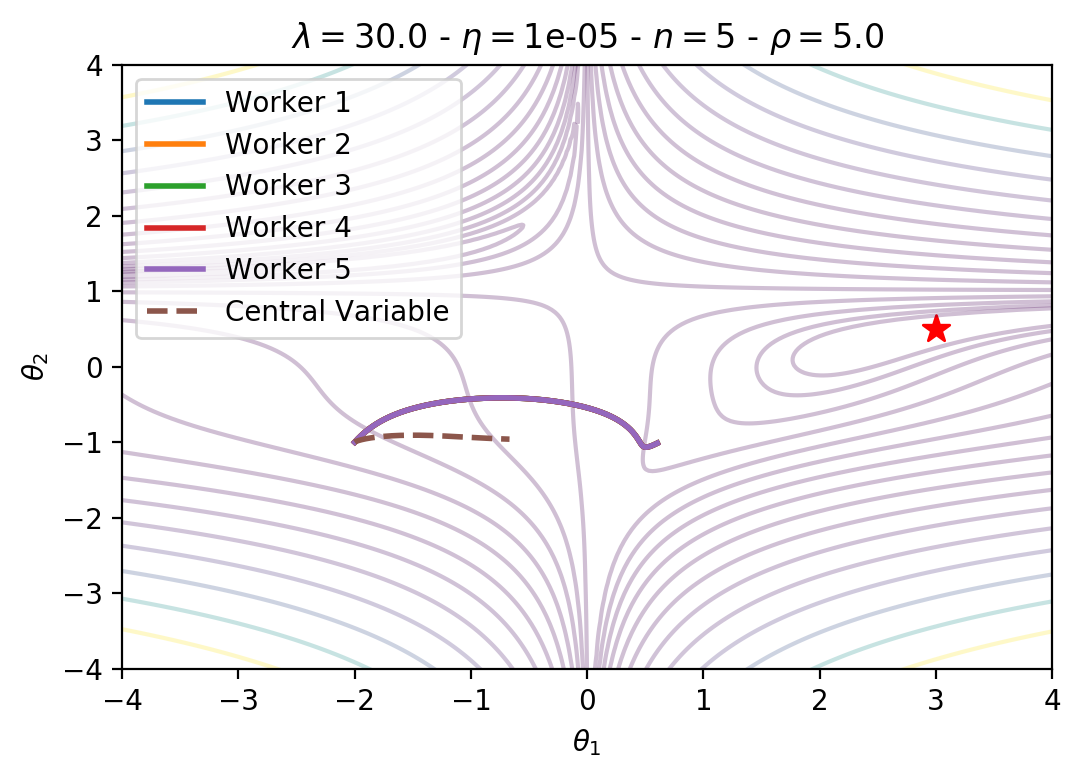
\includegraphics[width=\linewidth]{resources/images/easgd_sync_norm_space.png}
  \end{subfigure}
  \begin{subfigure}{.45\textwidth}
    \centering
    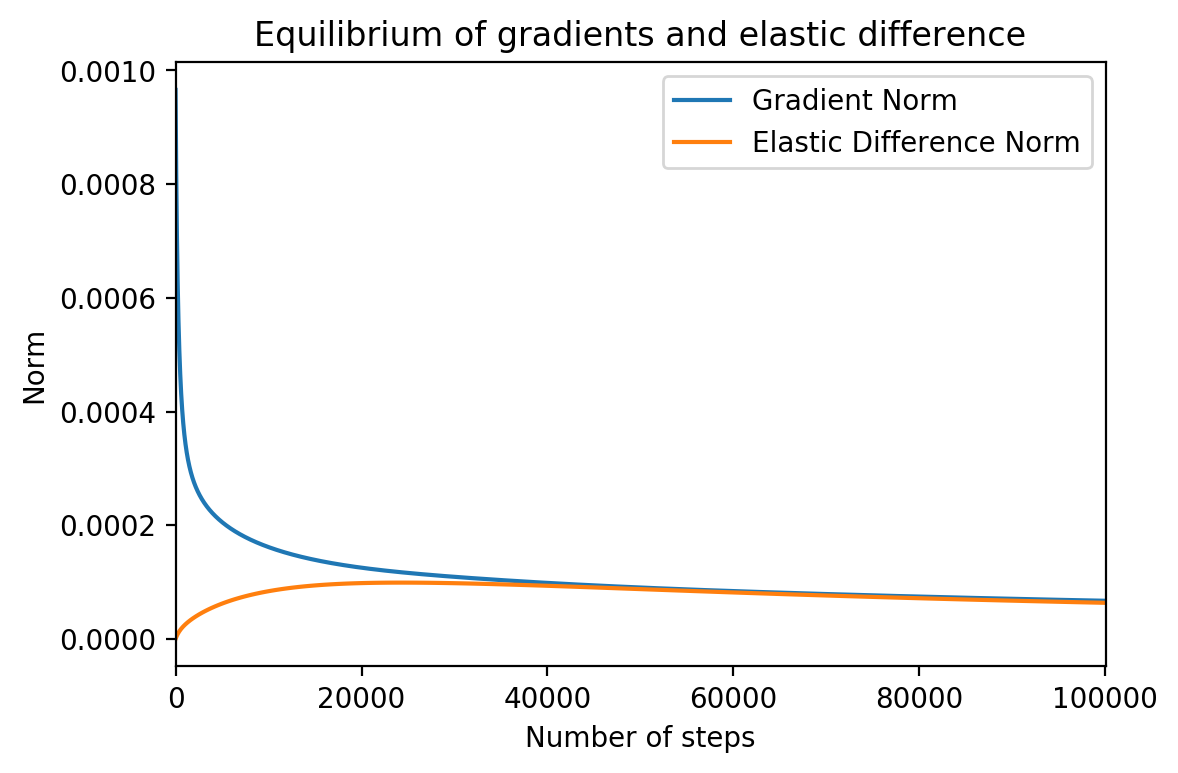
\includegraphics[width=\linewidth]{resources/images/easgd_sync_norm_equilibrium.png}
  \end{subfigure}
  \caption{In this experiment we use $\rho = 5$, as suggested by the authors~\cite{zhang2015deep}. We observe that at some point the elastic difference is starting to the influence the first-order gradients causing the workers to bend downwards, which is not present in Figure~\ref{fig:easgd_sync_equilibrium_small_rho}. This ``bend'' is due to a significant elastic force pointing in the direction of the central variable. If we would decompose the vector in its main components, i.e., $\theta_1$ and $\theta_2$, we would find that the $\theta_2$ component is significant enough to cause to worker to bend downwards since the elastic force is getting stronger proportional to the distance between the worker and the central variable and hyperparameter $\rho$. Furthermore, the equilibrium plot shows that the worker does a lot of initial exploration, while the central variable slowly follows the workers based on the averaged elastic difference. After 40000 steps, we see that the workers reach the equilibrium condition. As a result, any computational work done by the workers within a communication window is wasted since the distance between the workers and the central variable needs to grow smaller for the elastic force to shrink. However, because the elastic force is shrinking proportionally to the distance between the workers and the central variable, it allows the workers to explore \emph{slightly} more of the hypothesis space since the workers already met the equilibrium condition.}
  \label{fig:easgd_sync_equilibrium}
\end{figure}

\begin{figure}[H]
  \centering
  \begin{subfigure}{.45\textwidth}
    \centering
    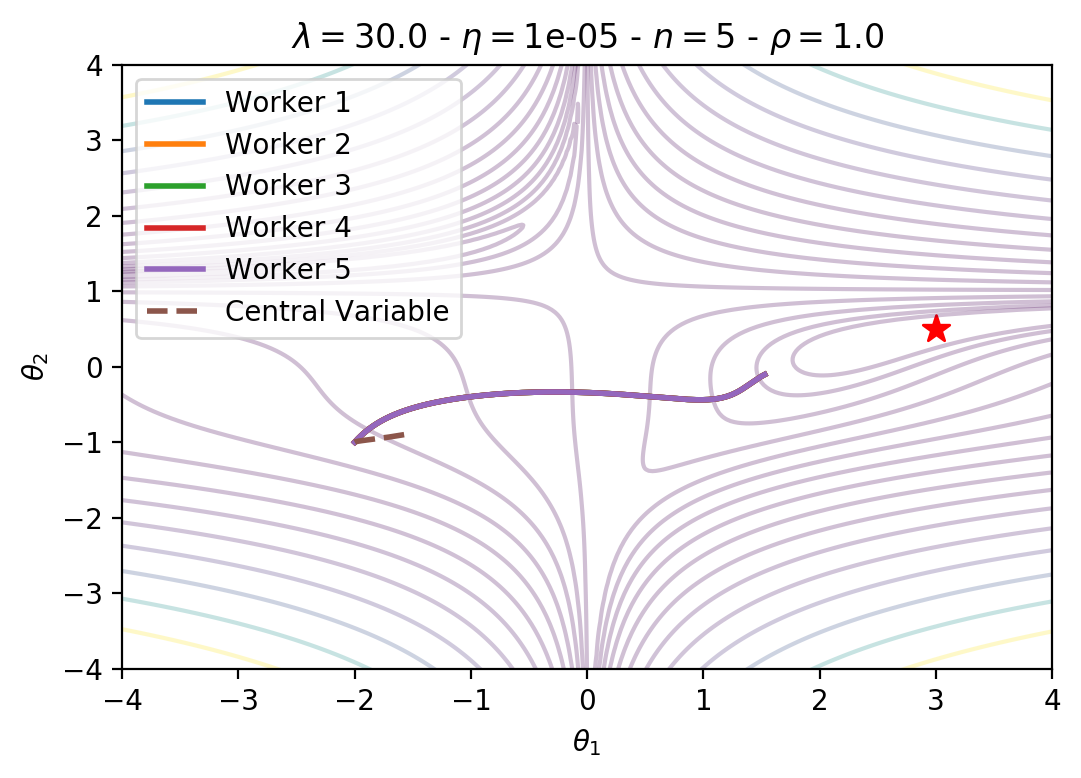
\includegraphics[width=\linewidth]{resources/images/easgd_sync_norm_space_2.png}
  \end{subfigure}
  \begin{subfigure}{.45\textwidth}
    \centering
    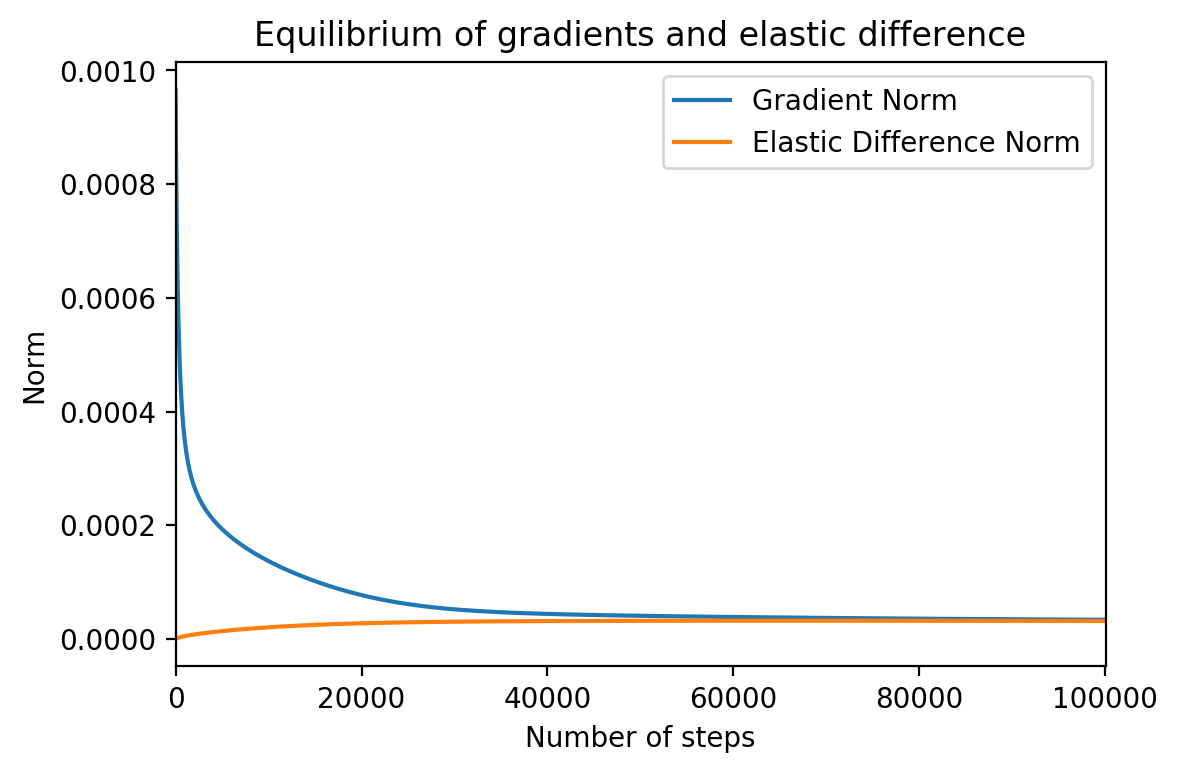
\includegraphics[width=\linewidth]{resources/images/easgd_sync_norm_equilibrium_2.png}
  \end{subfigure}
  \caption{In this experiment we reduce the value of the exploration hyperparameter $\rho$ while all other hyperparameters from our experiment in Figure~\ref{fig:easgd_sync_equilibrium} remain the same. After running the experiment we do not observe the ``bend'' which we initially observed in Figure~\ref{fig:easgd_sync_equilibrium}. However, this was expected since the elastic force is not that prominent due to the reduced value of hyperparameter $\rho$. Nevertheless, we still observe that the workers reach the equilibrium condition, with the difference that the central variable shows slower convergence behavior compared to Figure~\ref{fig:easgd_sync_equilibrium}.}
  \label{fig:easgd_sync_equilibrium_small_rho}
\end{figure}

To improve convergence of the central variable in \textsc{easgd}, and reduce the amount of wasted computational resources, we implemented Equation~\ref{eq:easgd_equilibrium_stopping_condition} based on Equation~\ref{eq:easgd_sync_working_condition} as a measure to stop wasting further computations.

\begin{equation}
  \label{eq:easgd_equilibrium_stopping_condition}
  \norm{-\eta_t \odot \nabla_\theta \mathcal{L}(\theta^k_t;\mathbf{x}^k_t;\mathbf{y}^k_t)} \leq \norm{\eta_t\rho(\theta^k_t - \tilde{\theta}_t)}
\end{equation}

However, we observed from our experiments that this exact condition is rarely satisfied. Of course, we made the assumption in Equation~\ref{eq:easgd_sync_equilibrium} that the parameterization of a worker does \emph{not} change if a worker settles in an equilibrium. Of course, before reaching the equilibrium, the gradient is non-zero, this implies that there is a change in the parameterization of a worker causing the elastic difference to be modified. With the result that the net force applied to the worker is \emph{approaching} the equilibrium. As a result, the net force applied to a worker is gradually becoming smaller.\\

In order to anticipate for a declining net force, and as a result, the gradually approaching equilibrium, we communicate the elastic difference with the parameter server if Equation~\ref{eq:easgd_equilibrium_fix} is met.

\begin{equation}
  \label{eq:easgd_equilibrium_fix}
  \Bigg(\norm{-\eta_t \odot \nabla_\theta \mathcal{L}(\theta^k_t;\mathbf{x}^k_t;\mathbf{y}^k_t)} - \norm{\eta_t\rho(\theta^k_t - \tilde{\theta}_t)}\Bigg) < \eta_t
\end{equation}

Using the same experimental configuration as in Figure~\ref{fig:easgd_sync_equilibrium}, with the difference that Equation~\ref{eq:easgd_equilibrium_fix} has been implemented as an early-stopping mechanism to communicate the elastic difference with the parameter server. Using Equation~\ref{eq:easgd_equilibrium_fix}, we can see that the proposed early stopping mechanism benefits the central variable in terms of convergence with respect to the default experimental configuration in Figure~\ref{fig:easgd_sync_equilibrium}.\\

What is remarkable about the equilibrium plot in Figure~\ref{fig:easgd_sync_fix} is the precense of a sudden drop in the norm of the elastic difference vector which is abscent in Figure~\ref{fig:easgd_sync_equilibrium} despite the fact that the workers follow similar paths. This is due to the early stopping mechanism which pulling the central variable closer towards the workers causing the decline in the norm of the elastic difference. Furthermore, since at this point the gradients are relatively small, a lot of local work can be done while at the same time the central variable will be able to keep the elastic distance small.

\begin{figure}[H]
  \centering
  \begin{subfigure}{.45\textwidth}
    \centering
    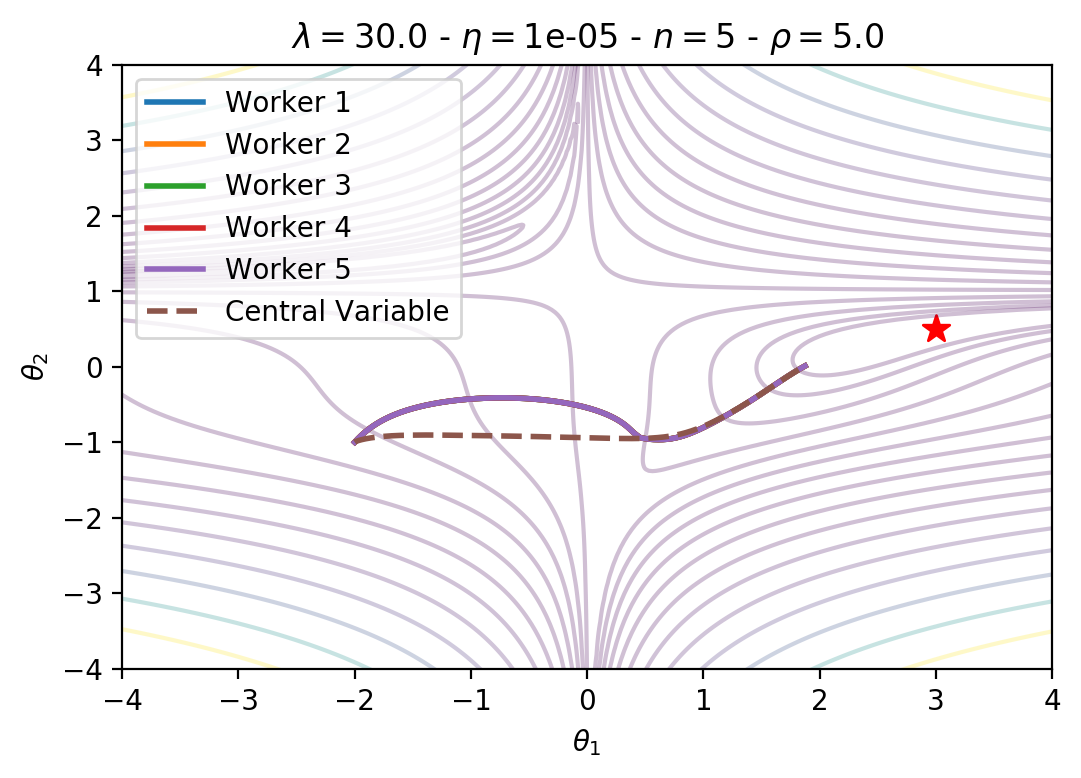
\includegraphics[width=\linewidth]{resources/images/easgd_sync_norm_space_fix.png}
  \end{subfigure}
  \begin{subfigure}{.45\textwidth}
    \centering
    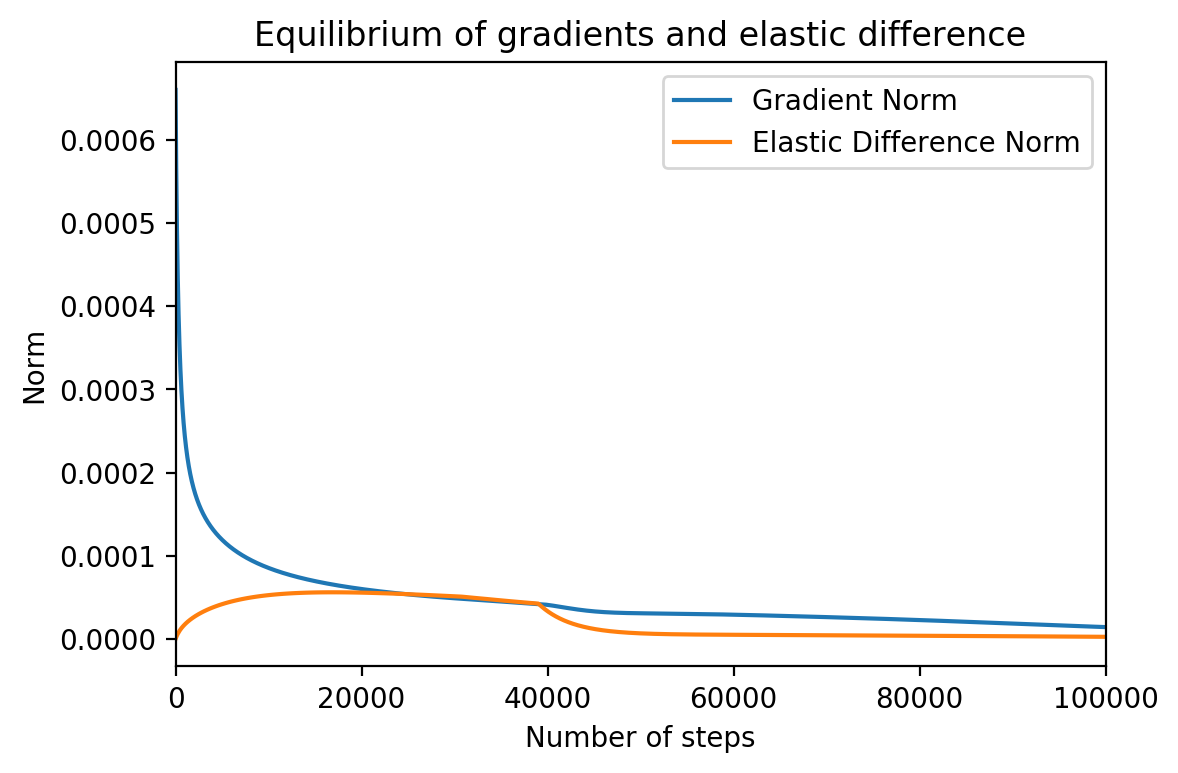
\includegraphics[width=\linewidth]{resources/images/easgd_sync_norm_ed_fix.png}
  \end{subfigure}
  \caption{\textsc{easgd} using the early stopping mechanism described in Equation~\ref{eq:easgd_equilibrium_fix}. Compared to Figure~\ref{fig:easgd_sync_equilibrium}, which uses the same experimental configuration, we observe that the central variable benefits in terms of convergence from increased communication when the early stopping condition is met.}
  \label{fig:easgd_sync_fix}
\end{figure}

Since the early stopping condition effectively communicates the elastic difference with the parameter server, is it not in essence increasing the communication frequency, i.e., lowering $\lambda$? In effect it isn't, since communication only takes place when the workers and the central variable approach an equilibrium condition. To show this, we conducted several experiments with and without the early stopping mechanism shown in Figure~\ref{fig:easgd_sync_lambda_10} and Figure~\ref{fig:easgd_sync_lambda_50}.

\begin{figure}[H]
  \centering
  \begin{subfigure}{.45\textwidth}
    \centering
    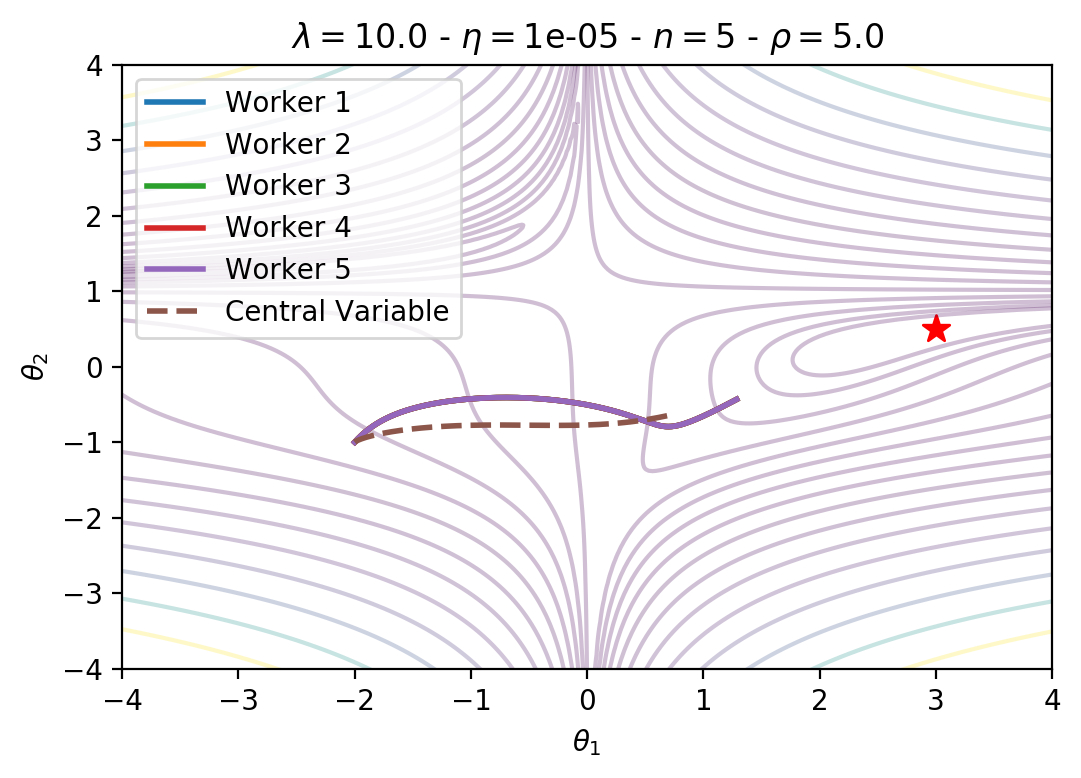
\includegraphics[width=\linewidth]{resources/images/easgd_es_10_n}
    \caption{No early stopping}
  \end{subfigure}
  \begin{subfigure}{.45\textwidth}
    \centering
    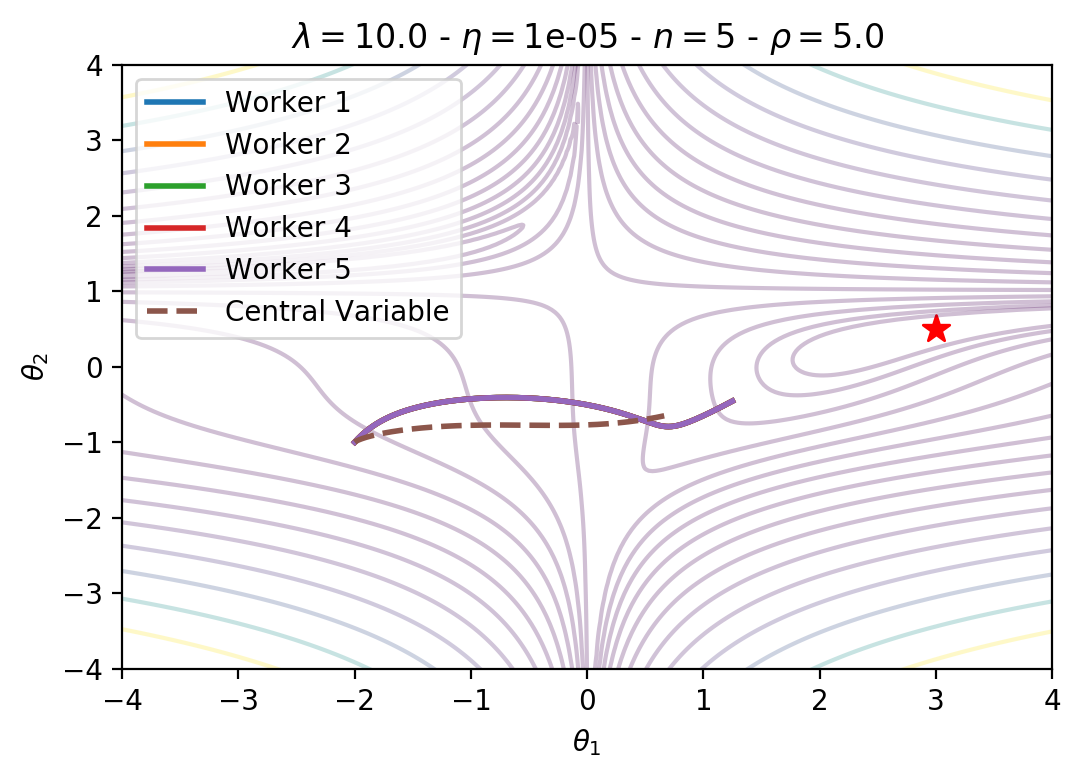
\includegraphics[width=\linewidth]{resources/images/easgd_es_10_y}
    \caption{Early stopping}
  \end{subfigure}
  \begin{subfigure}{.45\textwidth}
    \centering
    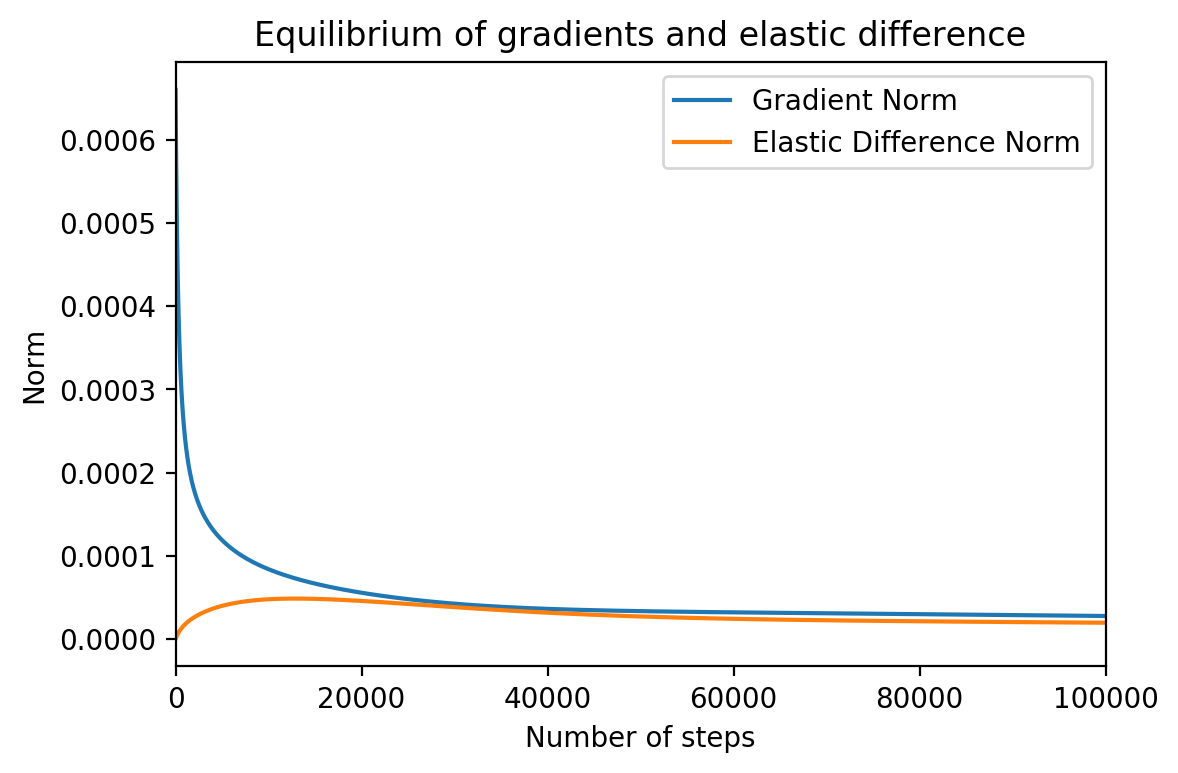
\includegraphics[width=\linewidth]{resources/images/easgd_es_10_n_eq}
    \caption{Equilibrium condition is not met (lines do not meet). As a result, early stopping is not applied.}
  \end{subfigure}
  \caption{$\lambda = 10$}
  \label{fig:easgd_sync_lambda_10}
\end{figure}

\begin{figure}[H]
  \centering
  \begin{subfigure}{.45\textwidth}
    \centering
    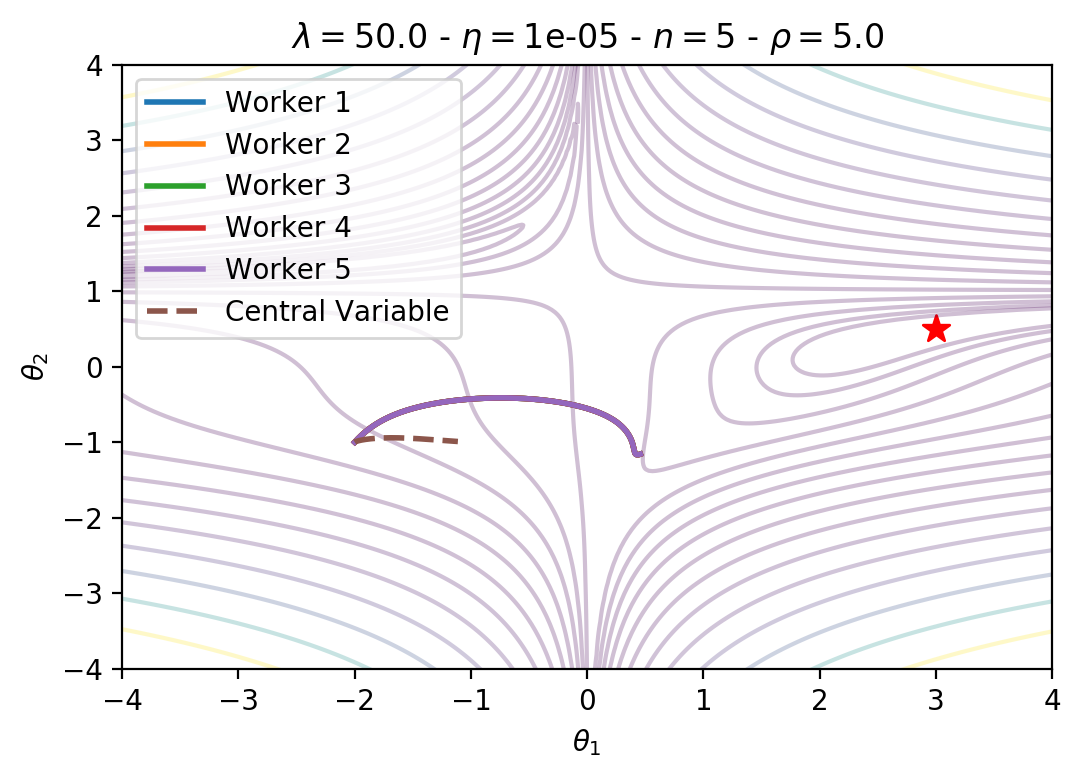
\includegraphics[width=\linewidth]{resources/images/easgd_es_50_n}
    \caption{No early stopping}
  \end{subfigure}
  \begin{subfigure}{.45\textwidth}
    \centering
    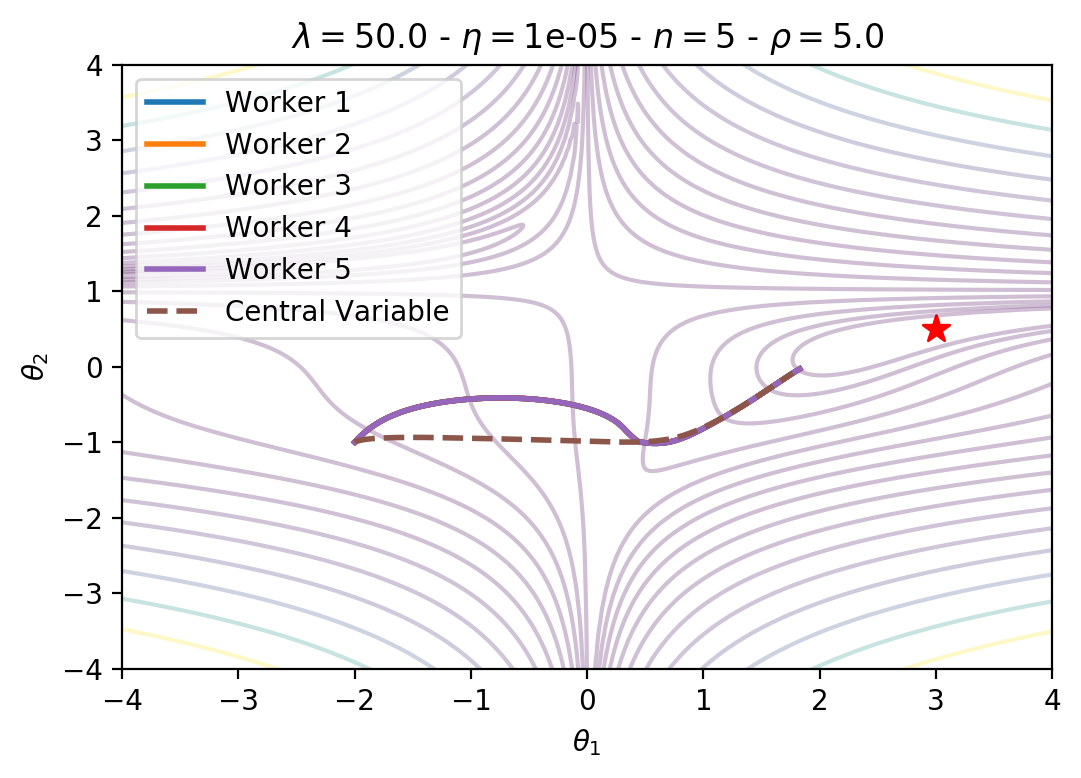
\includegraphics[width=\linewidth]{resources/images/easgd_es_50_y}
    \caption{Early stopping}
  \end{subfigure}
  \begin{subfigure}{.45\textwidth}
    \centering
    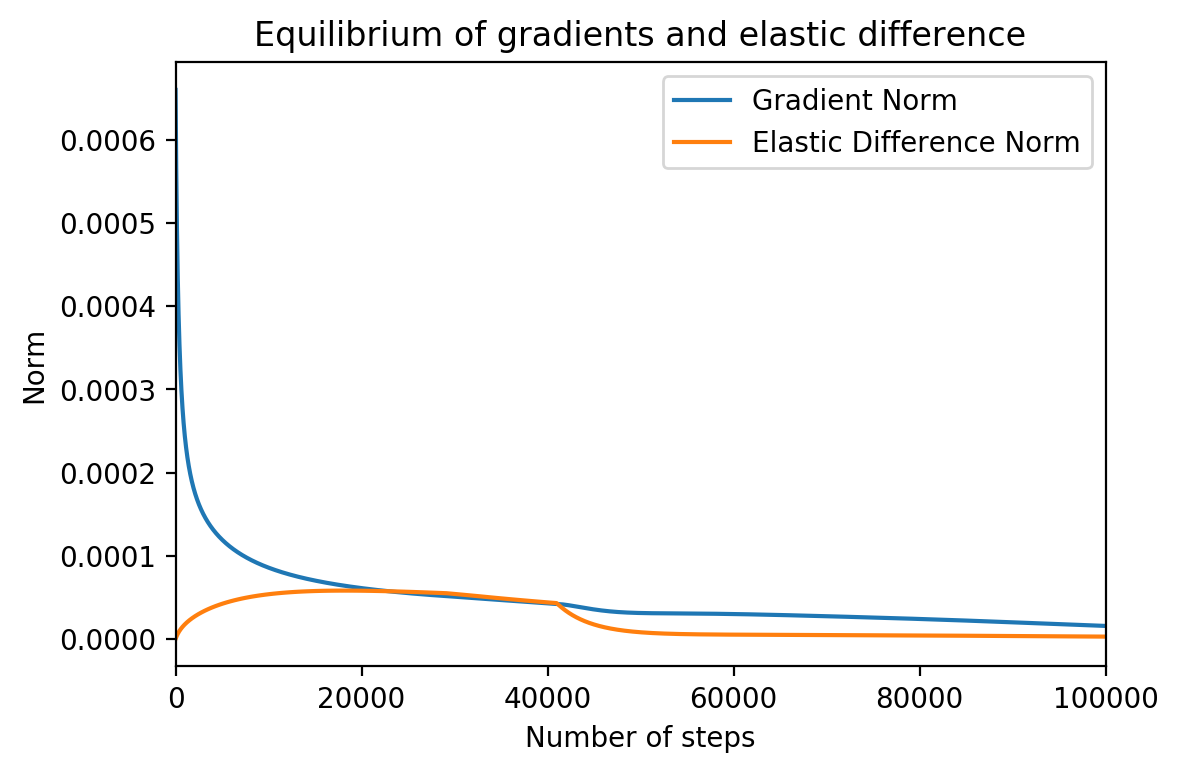
\includegraphics[width=\linewidth]{resources/images/easgd_es_50_y_eq}
    \caption{Equilibrium condition is met. Early stopping is applied.}
  \end{subfigure}
  \caption{$\lambda = 50$}
  \label{fig:easgd_sync_lambda_50}
\end{figure}

An other interesting phenomena is when \textsc{easgd} is approaching a minima. Compared to other synchronous optimizers such as mini-batch parallelism, or model averaging, \textsc{easgd} requires a significant amount of additional steps to actually converge to the minima because of the equilibrium condition as shown in Figure~\ref{fig:easgd_sync_slow}. Remember, if the workers are approaching the equilibrium condition, a small net force is applied to the worker because the \emph{negated} elastic difference counter-acts the advances of the workers to minimize the variance of the workers with respect to the central variable.

\begin{figure}[H]
  \centering
  \begin{subfigure}{.45\textwidth}
    \centering
    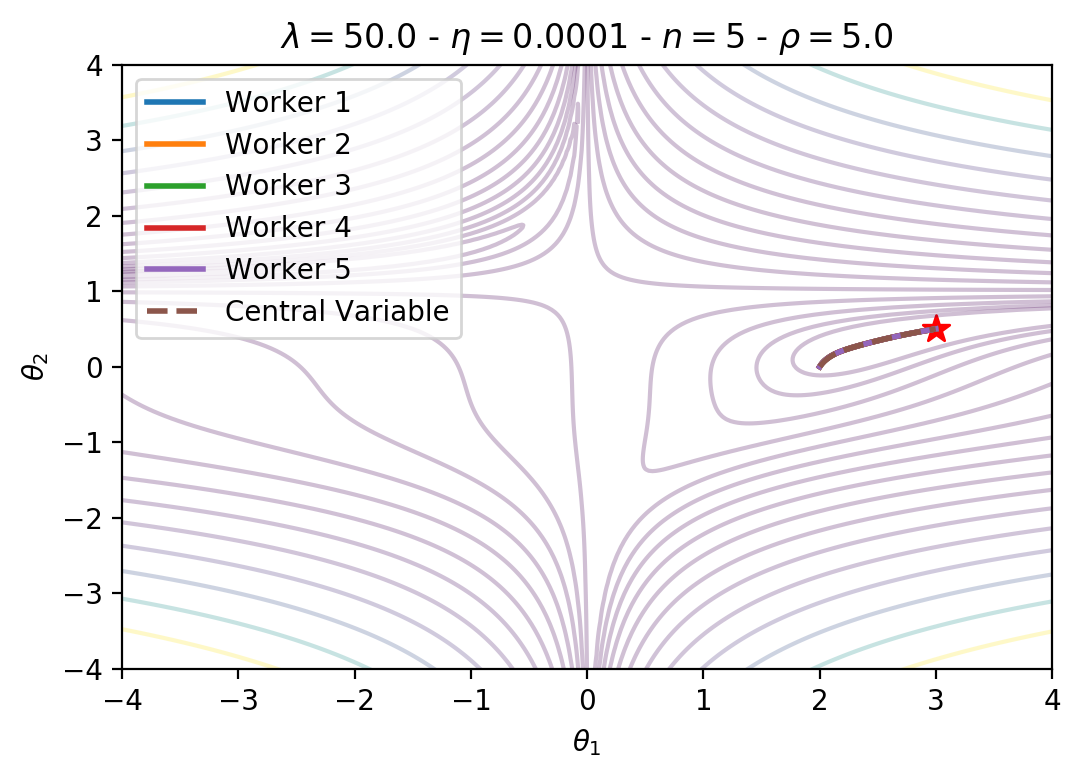
\includegraphics[width=\linewidth]{resources/images/easgd_sync_slow_space}
  \end{subfigure}
  \begin{subfigure}{.45\textwidth}
    \centering
    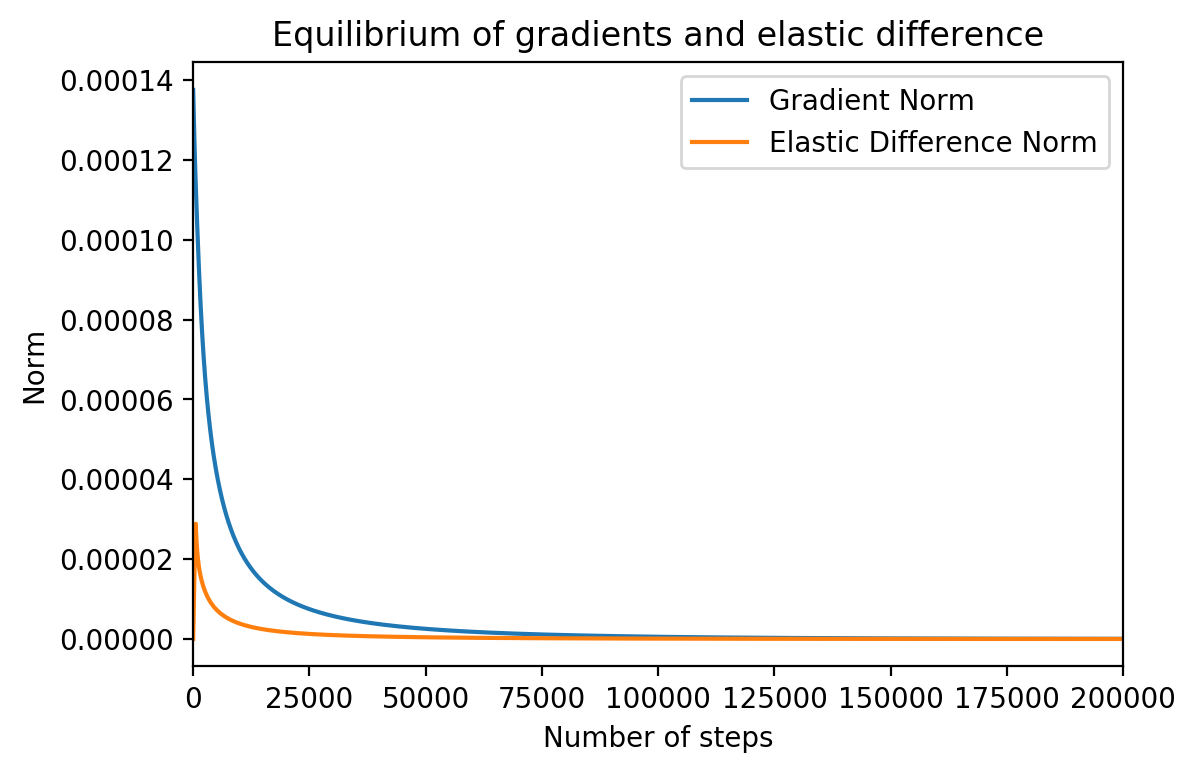
\includegraphics[width=\linewidth]{resources/images/easgd_sync_slow_eq}
  \end{subfigure}
  \caption{Slow converge of \textsc{easgd} at minima due to the equilibrium condition. In this figure we apply early stopping but due to the small gradients close to the minima it does not have any significant effects.}
  \label{fig:easgd_sync_slow}
\end{figure}

\section{Asynchronous Data Parallelism}
\label{sec:asynchronous_data_parallelism}

\subsection{DOWNPOUR}
\label{sec:downpour}

Waits induced by blocking mechanisms in synchronous data parallelism significantly reduce the harware utilisation during training, especially in non-homogeneous hardware configurations. As mentioned in Section~\ref{sec:ddl_introduction}, this can be resolved by simply removing the synchronizations barriers, as suggested by~\cite{dean2012large}. The algorithm the authors proposed is called \textsc{downpour}, and is shown in Algorithm~\ref{algo:downpour_worker}.\\

\textsc{downpour} is an intuitively a very simple algorithm. As before, we have $n$ different workers optimizing a central variable $\tilde{\theta}_t$ with the difference that every worker will \emph{commit} a gradient after every mini-batch in an asynchronous fashion, and after a commit has been performed, the worker will synchronize with the parameter server by \emph{pulling} the most recent parameterization of the central variable.

\begin{equation}
  \label{eq:downpour_worker}
  \theta^k_{t+1} = \theta^k_t - \eta_t \odot \nabla_\theta \mathcal{L}(\theta^k_t;\mathbf{x}^k_t;\mathbf{y}^k)
\end{equation}

\begin{equation}
  \label{eq:downpour_ps}
  \tilde{\theta}_{t+1} = \tilde{\theta}_t - \eta_t \odot \nabla_\theta \mathcal{L}(\theta^k_t;\mathbf{x}^k_t;\mathbf{y}^k)
\end{equation}

As mentioned in Chapter~\ref{chapter:introduction}, due to the asynchronous optimization one does not have the issue with idle workers due to synchronizations mechanisms. Instead, there is a more severe problem related to the parameterizations of the workers. Since workers will commit gradients to the central variable in an asynchronous manner, other workers will commit gradients based on older parameterizations of the central variable. As a result, the gradients of these workers are \emph{stale} as shown in Figure~\ref{fig:intro_asyn_data_parallelism} and Figure~\ref{fig:downpour_convergence}. An additional, but related issue to parameter staleness, is that increasing the amount of asynchronous workers, increases the staleness in the system as shown in Figure~\ref{fig:staleness_distribution}.

\begin{algorithm}[H]
  \caption{Worker procedure of \textsc{downpour}, which is a parallelized extension of \textsc{sgd}.}
  \label{algo:downpour_worker}
  \begin{algorithmic}[1]
    \Procedure{DOWNPOURWorker}{$k$}
    \State $\theta^k_0 \gets \tilde{\theta} \gets \Call{Pull}$
    \State $t \gets 0$
    \While{$\textbf{not}$ converged}
    \State $\textbf{x},~\textbf{y} \gets \Call{FetchNextMiniBatch()}{}$
    \State $g \gets -\eta_t \odot \nabla_\theta \mathcal{L}(\theta^k_t;\textbf{x};\textbf{y})$
    \State $\Call{Commit}{g}$
    \State $\theta^k_{t + 1} \gets \Call{Pull}$
    \State $t \gets t + 1$
    \EndWhile
    \EndProcedure
  \end{algorithmic}
\end{algorithm}

Nevertheless, contrary to \textsc{easgd}, \textsc{downpour} is not designed with communication constraints in mind. As a result, increasing the number of workers in an already saturated environment will not reduce the training time since whenever a worker computes a gradient, it will commit the result to the parameter server. To illustrate this, imagine having several workers committing highly dimensional gradients to the parameter server. Since it takes some time to incorperate these gradients into the central variable, other workers will have to wait for their turn in the queue. To reduce the side-effects (waits) in this particular situation,~\cite{louppe2010zealous} proposes to before committing the gradient, a worker should send a small control message to check if the queue is currently occupied, i.e., gradients of other workers are being incorperated into the central variable. If this is the case, do not commit the gradient, but fetch the next mini-batch, compute the gradient, and accumulate the computed gradient with the previously computed gradient, and send a new control message\\

An obvious problem with this method is that the possibility exists that after $x$ number of retries, the central variable queue is still occupied by other workers. Following the naive procedure, the zealous method should keep accumulating new gradients. However, this is problematic at step $x + 1$, when the queue is available. Imagine the possibility that other workers, and the central variable converged to a different minima. If our worker would commit the accumulated gradient in this particular situation, then the central variable would not be close to its minima as it was before. In order to reduce the amount of staleness in such a situation, one could introduce a limit to the amount of local steps that can be made in an attempt to reduce staleness as shown in Algorithm~\ref{algo:downpour_worker_zealous}.\\

However, this technique introduces an additional hyperparameter. Several other approaches which handle this problem in a different way without introducing new hyperparameters, and additionally giving some intuition and insight into parameter staleness in Deep Learning are discussed in detail in Chapter~\ref{chapter:accumulated_gradient_normalization} and Chapter~\ref{chapter:asynchronous_distributed_adaptive_gradients}.

\begin{algorithm}[H]
  \caption{Zealous worker procedure of \textsc{downpour}, inspired by~\cite{louppe2010zealous}.}
  \label{algo:downpour_worker_zealous}
  \begin{algorithmic}[1]
    \Procedure{ZealousDOWNPOURWorker}{$k$}
    \State $\theta^k_0 \gets \tilde{\theta} \gets \Call{Pull}$
    \State $t \gets 0$
    \While{$\textbf{not}$ converged}
    \State $i \gets 0$
    \State $g \gets 0$
    \While{$i < \lambda$}
    \State $\textbf{x},~\textbf{y} \gets \Call{FetchNextMiniBatch()}{}$
    \State $g \gets g -\eta_t \odot \nabla_\theta \mathcal{L}(\theta^k_t;\textbf{x};\textbf{y})$
    \If{$\textbf{not}$~\Call{QueueOccupied}~~$\textbf{or}$~$i = (\lambda -1)$}
    \State $\Call{Commit}{g}$
    \State $\theta^k_{t + 1} \gets \Call{Pull}$
    \State $i \gets \lambda$ \Comment{Satisfy stopping condition.}
    \EndIf
    \State $t \gets t + 1$
    \State $i \gets i + 1$
    \EndWhile
    \EndWhile
    \EndProcedure
  \end{algorithmic}
\end{algorithm}

\begin{figure}[H]
  \centering
  \begin{subfigure}{.49\textwidth}
    \centering
    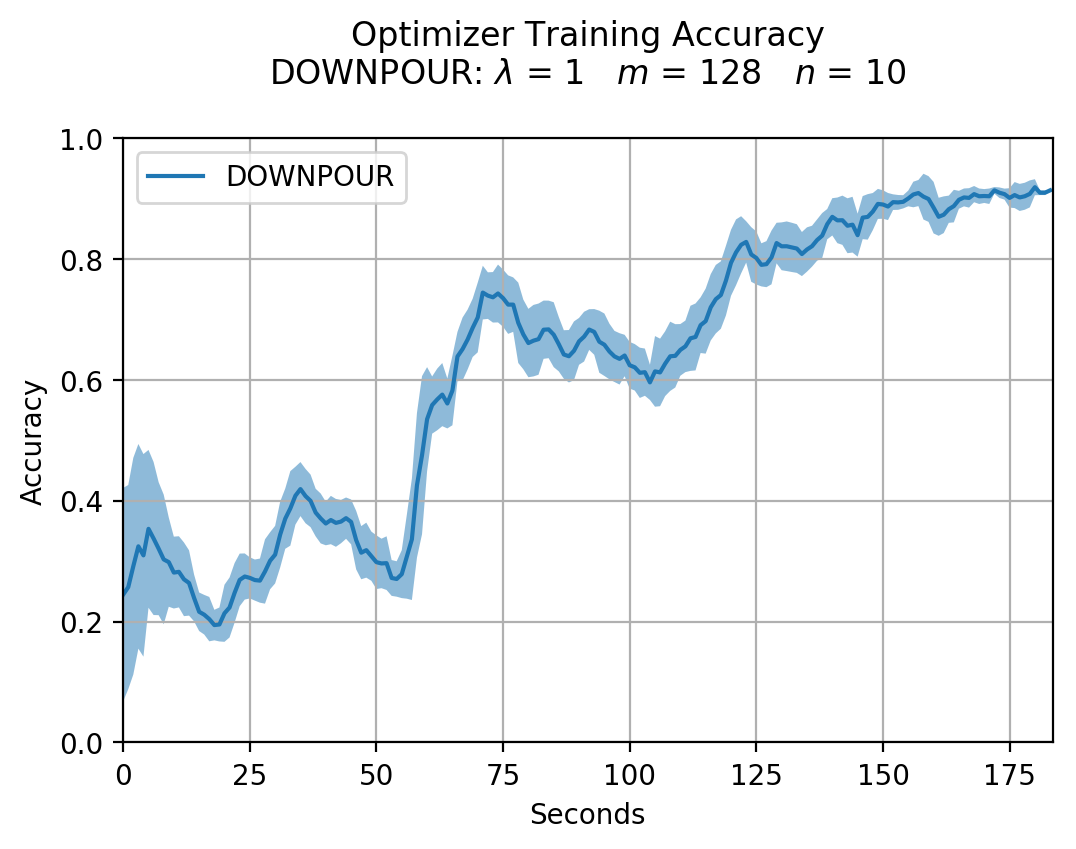
\includegraphics[width=\linewidth]{resources/images/downpour_10}
    \caption{$n = 10$}
  \end{subfigure}
  \begin{subfigure}{.49\textwidth}
    \centering
    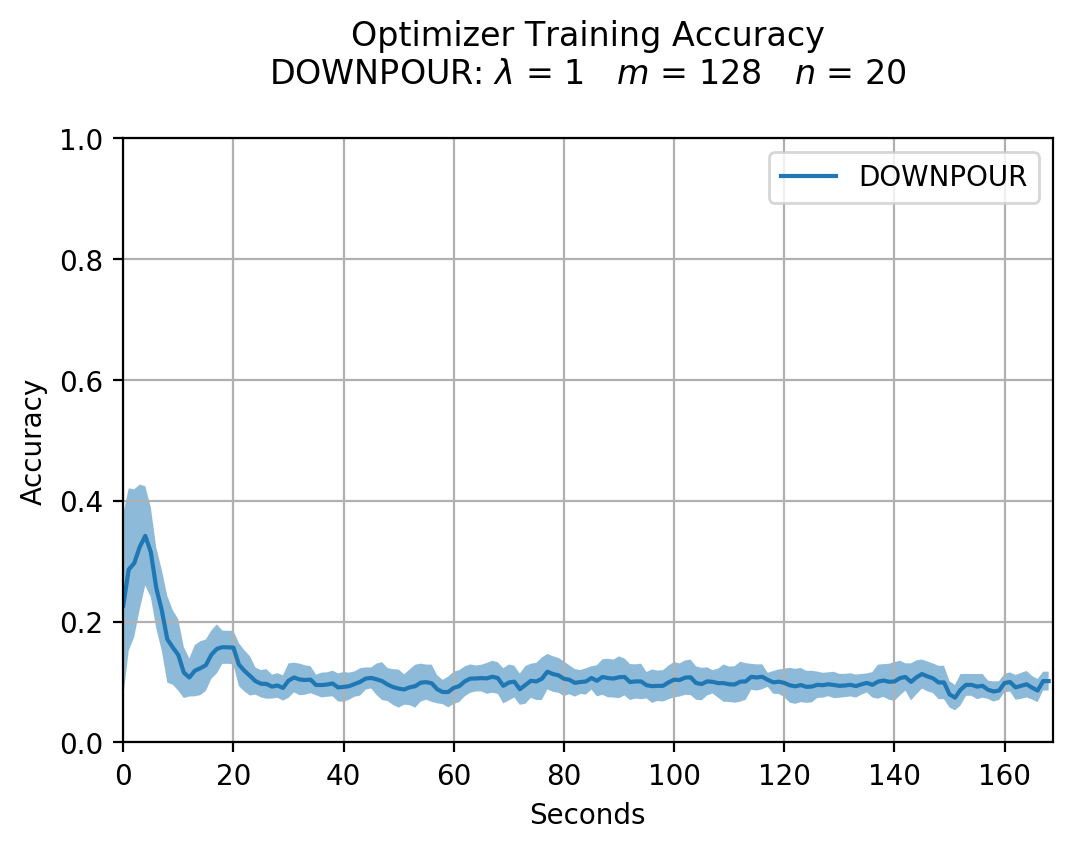
\includegraphics[width=\linewidth]{resources/images/downpour_20}
    \caption{$n = 20$}
  \end{subfigure}
  \caption{Divergence due to number ($n = 20$) of asynchronous workers in the optimization process~\cite{implicitmomentum} and not dealing with parameter staleness in a more intelligent way. Lowering the number workers ($n = 10$) causes the central variable to converge.}
  \label{fig:downpour_convergence}
\end{figure}


\subsection{Dynamic SGD}
\label{sec:dyn_sgd}

The intrinsic reason that asynchronous methods like \textsc{downpour} cannot guarentee convergence is that these method directly incorperate local updates (good) and stale updates (bad) in the central variable~\cite{jiang2017heterogeneity}. To combat this, one could incorperate staleness information of a worker to have a per-worker learning which decays protentionally stale gradients proportional to the staleness~\cite{jiang2017heterogeneity}. As a result, Equation~\ref{eq:dynsgd_ps} will better cope with parameter staleness in contrast to \textsc{downpour}.

\begin{equation}
  \label{eq:dynsgd_ps}
  \tilde{\theta}_{t+1} = \tilde{\theta}_t - \frac{\eta_t}{\tau_i} \odot \nabla_\theta \mathcal{L}(\theta^k_t;\mathbf{x}^k_t;\mathbf{y}^k_t)
\end{equation}

However, we would like to note that in a homogeneous hardware configuration the gradients will be scaled down proportional to the number of asynchronous workers as $\mathbf{E}[\tau] = (n - 1)$~\cite{implicitmomentum}. As a result, the expected scalar that will be applied to a worker gradient in a homogeneous setting is summarized in Equation~\ref{eq:dynsgd_homogeneous}.

\begin{equation}
  \label{eq:dynsgd_homogeneous}
  \mathbf{E}\Bigg[\frac{1}{\tau}\Bigg] = \Bigg(\frac{1}{n - 1}\Bigg)
\end{equation}

Furthermore, as we will see in Chapter~\ref{chapter:asynchronous_distributed_adaptive_gradients}, this technique scales down gradients with respect to the number of stale steps, while the issue of staleness mainly arrises from the \emph{distance between parameterizations}. For example, imagine a plateau where the workers have to pass through in order to converge to a minima. Since progress is slow in a plateau, thus the distance between the workers and the central variable will remain relatively small, it is non-sensical to scale down the gradients with respect to the number of stale steps, since these gradients provide good information because they are \emph{close to the ``old'' central variable}.\\

Nevertheless, in order to capture the staleness information, some additional engineering is required to keep track of worker staleness since the worker themselves to not possess this information. Contrary to~\cite{jiang2017heterogeneity}, we propose a different architecture to capture the staleness information. In our approach we exchange messages between the parameters server and workers. These messages can obtain additional information beside the parameterization of a worker or the central variable. During the initialization phase of the training procedure, we keep track of a \emph{parameter server clock}. Basically, this clock holds the number of updates that have been applied to the central variable. Furthermore, in order to obtain the staleness of every worker, and apply the scaling factor described in Equation~\ref{eq:dynsgd_ps}, the parameter server needs to keep track of the last \emph{clock tick} when a worker $i$ sent an update. It does so by maintaining a hashmap, or a different datastructure, to associate the last update clock tick with a particular worker. Furthermore, we scale the parameterizations on the parameter server since this will ensure the consistency of the staleness information because it is possible that an other worker might commit an update in the meantime (CAP theorem), and reduce the amount of blocking mechanisms. Nevertheless, for (very) large networks there might be an issue when insufficient processing power is allocated to preprocess the queue in an efficient manner.\\

An additional requirement of this architecture, is that the parameter server needs to update the worker datastructure whenever a worker \emph{pulls} the central variable (because the worker will compute a gradient based on the parameterization of the central variable it just pulled, and this is required to compute the number of updates that happened in between). Then, whenever a worker commits a gradient to the central variable, the paramter server just needs the compute the difference between the last recorded clock time of this particular worker and the current value of the parameter server clock. Where the last recorded clock tick of a particular worker can be retrieved from the data structure mentioned above. The complete pseudo-code for these procedures can be found in Algorithm~\ref{algo:dynsgd_worker} and Algorithm~\ref{algo:dynsgd_parameter_server}.

\newpage

\begin{algorithm}[H]
  \caption{Worker procedure of \textsc{dynsgd}.}
  \label{algo:dynsgd_worker}
  \begin{algorithmic}[1]
    \Procedure{DynSGDWorker}{$k$}
    \State $\theta^k_0 \gets \tilde{\theta} \gets \Call{Pull}$
    \State $t \gets 0$
    \While{$\textbf{not}$ converged}
    \State $i \gets 0$
    \State $g \gets 0$
    \While{$i < \lambda$}
    \State $\textbf{x},~\textbf{y} \gets \Call{FetchNextMiniBatch()}{}$
    \State $g \gets g -\eta_t \odot \nabla_\theta \mathcal{L}(\theta^k_t;\textbf{x};\textbf{y})$
    \If{$\textbf{not}$~\Call{QueueOccupied}~~$\textbf{or}$~$i = (\lambda -1)$}
    \State $\Call{Commit}{g}$
    \State $\theta^k_{t + 1} \gets \Call{Pull}$
    \EndIf
    \State $t \gets t + 1$
    \State $i \gets i + 1$
    \EndWhile
    \EndWhile
    \EndProcedure
  \end{algorithmic}
\end{algorithm}

\begin{algorithm}[H]
  \caption{Parameter server procedures of \textsc{dynsgd}.}
  \label{algo:dynsgd_parameter_server}
  \begin{algorithmic}[1]
    \Procedure{DynSGDParameterServer}{}
    \State $\tilde{c} \gets 0$ \Comment{Parameter server clock}
    \State $\tilde{m} \gets \tilde{c}$ \Comment{Initialize staleness datastructure}
    \Procedure{HandlePull}{$k$} \Comment{$k$ denotes the worker identifier}
    \State $\tilde{m}[k] = \tilde{c}$
    \State \Return $\tilde{\theta}_{\tilde{c}}$
    \EndProcedure
    \Procedure{HandleCommit}{$k$, $\Delta\theta^k$}
    \State $\tau \gets \tilde{c} - \tilde{m}[k]$
    \State $\tilde{\theta}_{\tilde{c} + 1} = \tilde{\theta}_{\tilde{c}} + \frac{1}{\tau + 1} \odot \Delta\theta^k$  \Comment{$+1$ to prevent division by 0}
    \State $\tilde{c} \gets \tilde{c} + 1$
    \EndProcedure
    \EndProcedure
  \end{algorithmic}
\end{algorithm}

\subsection{Asynchronous Elastic Averaging SGD}
\label{sec:aeasgd}

\section{Hybrids}
\label{sec:hybrids}
